\documentclass[12pt,a4paper]{article}

% =============================
% XeLaTeX + Unicode
% =============================
\usepackage{fontspec}
\usepackage{polyglossia}
\setdefaultlanguage{vietnamese}



% Font chữ: ưu tiên font có hỗ trợ đầy đủ tiếng Việt.
% =============================
% Font chữ: Latin Modern
% =============================
\setmainfont{Latin Modern Roman}
\setsansfont{Latin Modern Sans}
\setmonofont{Latin Modern Mono}

% =============================
% Packages cơ bản
% =============================
\usepackage{tikz}
\usetikzlibrary{arrows.meta, positioning, calc, shapes.geometric, automata, backgrounds, fit}
\usepackage{array}
\usepackage{multirow}
\usepackage{float}
\usepackage{booktabs}
\usepackage{caption}
\usepackage{tabularx}
\usepackage[table]{xcolor}
\usepackage{amsmath, amssymb}
\usepackage{graphicx}
\graphicspath{{./}{asset/}}
\usepackage{titlesec}
\usepackage{ragged2e}
\usepackage{etoolbox}
\usepackage{xurl}
\usepackage{pdfpages}
\usetikzlibrary{fit}
% =============================
% Canh lề
% =============================
\newcolumntype{Y}{>{\raggedright\arraybackslash}X}
\newcolumntype{L}[1]{>{\raggedright\arraybackslash}p{#1}}
\usepackage[a4paper,margin=2.5cm]{geometry}

% =============================
% Thụt đầu dòng
% =============================
\setlength{\parindent}{1.27cm}
\usepackage{indentfirst}

% =============================
% Giãn dòng
% =============================

\usepackage{setspace}
\onehalfspacing


\titleformat{\section}
  {\normalfont\Large\bfseries}{\thesection}{0.75em}{}
\titleformat{\subsection}
  {\normalfont\large\bfseries}{\thesubsection}{0.75em}{}
\titleformat{\subsubsection}
  {\normalfont\normalsize\bfseries}{\thesubsubsection}{0.75em}{}
\titlespacing*{\section}{0pt}{18pt}{12pt}
\titlespacing*{\subsection}{0pt}{14pt}{8pt}
\titlespacing*{\subsubsection}{0pt}{10pt}{6pt}

\setcounter{secnumdepth}{4}
\setcounter{tocdepth}{2}

% =============================
% List
% =============================
\usepackage{enumitem}
\setlist[itemize,1]{label=\textbullet}
\setlist[itemize,2]{label=$\circ$}
\setlist[itemize]{leftmargin=1.5em}

% =============================
% Hyperref
% =============================
\usepackage{hyperref}
\hypersetup{
  colorlinks=true,
  linkcolor=black,
  urlcolor=cyan
}
\usepackage{listings}

% Định nghĩa màu sắc cho giống các trình soạn thảo code HDL
\definecolor{vgreen}{RGB}{0,120,0}
\definecolor{vblue}{RGB}{0,0,255}
\definecolor{vorange}{RGB}{255,150,0}

\lstset{
    language=Python,
    basicstyle=\small\ttfamily,
    keywordstyle=\color{vblue}\bfseries,
    commentstyle=\color{vgreen},
    stringstyle=\color{vorange},
    numbers=left,
    numberstyle=\tiny\color{gray},
    stepnumber=1,
    frame=single,
    breaklines=true,
    tabsize=4
}

\newcommand{\todoimage}[2][0.9\textwidth]{%
    \fbox{%
        \begin{minipage}[c][4cm][c]{#1}
            \centering
            \textbf{TODO:} #2
        \end{minipage}%
    }%
}

\begin{document}

% ===== FRONT MATTER =====
\begin{titlepage}
\thispagestyle{empty}

\begin{center}
    \fontsize{14}{16}\selectfont
    \textbf{ĐẠI HỌC QUỐC GIA TP. HỒ CHÍ MINH}\\
    \textbf{TRƯỜNG ĐẠI HỌC CÔNG NGHỆ THÔNG TIN}
\end{center}

\vspace{1cm}

\begin{center}
    
\includegraphics[width=6cm]{uit_logo.png}
\end{center}

\vspace{1cm}

\begin{center}
    \fontsize{13}{15}\selectfont
    \textbf{KHOA: KỸ THUẬT MÁY TÍNH}\\
    \vspace{0.3cm}
    \textbf{MÔN HỌC: CE224.Q11}
\end{center}

\vspace{1cm}

\hrule
\vspace{0.3cm}

\begin{center}
    \fontsize{15}{20}\selectfont
    \textbf{HỆ THỐNG KHÓA CỬA THÔNG MINH\\
    NHẬN DIỆN KHUÔN MẶT KẾT HỢP FUZZY LOGIC}
\end{center}

\vspace{0.3cm}
\hrule

\vspace{1cm}

\begin{spacing}{1.4}
\noindent
\makebox[\textwidth]{%
\begin{minipage}{0.62\textwidth}
\textit{Sinh viên thực hiện:}\\[0.3cm]
Nguyễn Hữu Minh Chiến -- 23520183\\
Phùng Minh Chí -- 23520179\\
Nguyễn Lê Minh Anh -- 23520063
\end{minipage}
\hfill
\begin{minipage}{0.33\textwidth}
\raggedleft
\textit{Giảng viên hướng dẫn:}\\[0.3cm]
ThS. Phạm Minh Quân
\end{minipage}}
\end{spacing}

\vfill

\begin{center}
    TP. Hồ Chí Minh, \the\year
\end{center}

\end{titlepage}


\section*{Tóm tắt}
\addcontentsline{toc}{section}{Tóm tắt}

Báo cáo trình bày quá trình xây dựng hệ thống khóa cửa thông minh \textbf{SmartLock Fuzzy}. Hệ thống sử dụng camera cục bộ để phát hiện và nhận diện khuôn mặt, kết hợp mô hình suy luận mờ Mamdani để đánh giá mức rủi ro truy cập. Kết quả suy luận được dùng để quyết định mở khóa, yêu cầu xác thực bổ sung, từ chối truy cập hoặc khóa tạm thời. Bên cạnh nhận diện khuôn mặt, hệ thống còn hỗ trợ xác thực bằng mã PIN qua keypad ma trận, hiển thị trạng thái trên màn hình OLED và điều khiển chốt khóa bằng servo.

Phần mềm được chia thành hai khối chính. Backend FastAPI chạy trên thiết bị cục bộ, trực tiếp đọc camera, xử lý ảnh bằng OpenCV, quản lý đăng ký khuôn mặt, điều khiển phần cứng Raspberry Pi và cung cấp API cho giao diện web. Frontend Next.js hiển thị luồng camera, kết quả nhận diện, mức rủi ro fuzzy, tiến trình đăng ký khuôn mặt và giao diện đổi mật khẩu keypad. Toàn bộ pipeline được thiết kế theo hướng hoạt động cục bộ, hạn chế phụ thuộc cloud và phù hợp với bối cảnh hệ thống nhúng.

Báo cáo tập trung mô tả kiến trúc, thuật toán, thiết kế API, luồng xử lý thời gian thực, giao tiếp phần cứng và các điểm cần kiểm chứng thực nghiệm. 
\clearpage


\tableofcontents
\clearpage
\listoffigures
\clearpage
\listoftables
\clearpage

% ===== CHAPTERS =====
\section{Tổng quan đề tài}

\subsection{Lý do chọn đề tài}

Trong bối cảnh các hệ thống thông tin ngày càng phát triển, nhu cầu tự động nhận diện và quản lý danh tính người dùng từ dữ liệu hình ảnh ngày càng trở nên quan trọng. Các phương pháp truyền thống như mật khẩu hoặc mã định danh tồn tại nhiều hạn chế, từ đó thúc đẩy sự phát triển của các phương pháp sinh trắc học, trong đó khuôn mặt là đặc trưng nổi bật nhờ tính tự nhiên và dễ sử dụng.


Các hệ thống kiểm soát ra vào truyền thống thường dựa trên chìa khóa cơ, thẻ từ hoặc mã PIN. Những phương pháp này dễ triển khai nhưng tồn tại nhiều hạn chế: chìa khóa có thể bị mất, thẻ có thể bị sao chép, còn mã PIN có thể bị lộ nếu người dùng thao tác trong môi trường không an toàn. Trong khi đó, camera và các bộ xử lý nhúng như Raspberry Pi ngày càng phổ biến, cho phép triển khai nhận diện khuôn mặt trực tiếp tại biên với chi phí thấp \cite{raspberrypi}.

Đề tài SmartLock Fuzzy được xây dựng nhằm kết hợp ba hướng kỹ thuật:

\begin{itemize}
    \item \textbf{Thị giác máy tính cục bộ}: camera được xử lý bằng OpenCV ngay trên thiết bị, không cần gửi ảnh lên máy chủ ngoài \cite{opencv}.
    \item \textbf{Ra quyết định bằng fuzzy logic}: thay vì chỉ dựa vào một ngưỡng cứng của mô hình nhận diện, hệ thống xét thêm điều kiện ánh sáng và góc mặt để đánh giá rủi ro \cite{zadeh1965}.
    \item \textbf{Tích hợp phần cứng nhúng}: keypad, OLED và servo giúp hệ thống hoạt động như một khóa cửa hoàn chỉnh chứ không chỉ là phần mềm demo.
\end{itemize}

Việc kết hợp nhận diện khuôn mặt với fuzzy logic phù hợp với bài toán khóa cửa vì dữ liệu camera luôn chịu ảnh hưởng của môi trường. Một khuôn mặt đúng người nhưng quá tối, quá sáng hoặc quay lệch nhiều không nên được xử lý giống như một khuôn mặt rõ, nhìn thẳng và có độ tin cậy cao.

\subsection{Mục tiêu đề tài}

Đề tài đặt ra các mục tiêu chính sau:

\begin{enumerate}
    \item Xây dựng backend FastAPI đọc camera cục bộ và cung cấp API cho frontend.
    \item Phát hiện khuôn mặt bằng Haar Cascade và nhận diện danh tính bằng LBPH.
    \item Ước lượng các đặc trưng hỗ trợ quyết định gồm độ sáng khuôn mặt, góc lệch tương đối và độ tin cậy nhận diện.
    \item Thiết kế bộ điều khiển fuzzy logic để ánh xạ các đặc trưng đầu vào thành mức rủi ro truy cập.
    \item Tích hợp keypad 4x4, OLED SSD1306 và servo trên Raspberry Pi.
    \item Xây dựng giao diện Next.js để quan sát camera, đăng ký khuôn mặt và đổi mật khẩu keypad.
    \item Cung cấp script huấn luyện/đánh giá mô hình và công cụ benchmark pipeline.
\end{enumerate}

\subsection{Phương pháp thực hiện}

Quy trình thực hiện được chia thành các giai đoạn:

\begin{enumerate}
    \item \textbf{Khảo sát và thiết kế kiến trúc}: xác định các thành phần backend, frontend, xử lý ảnh, fuzzy logic và phần cứng.
    \item \textbf{Xây dựng pipeline camera}: đọc frame từ camera, phát hiện khuôn mặt, nhận diện bằng LBPH và mã hóa ảnh JPEG để gửi lên dashboard.
    \item \textbf{Thiết kế bộ fuzzy}: định nghĩa biến ngôn ngữ, hàm thành viên Gaussian, tập luật Mamdani và ngưỡng ánh xạ hành động.
    \item \textbf{Tích hợp đăng ký khuôn mặt}: thu thập mẫu hợp lệ, lọc ảnh mờ/thiếu sáng/góc lệch, huấn luyện lại mô hình LBPH và nạp lại model khi chạy.
    \item \textbf{Tích hợp phần cứng}: quét keypad bằng interrupt, điều khiển servo bằng PWM và cập nhật trạng thái OLED.
    \item \textbf{Xây dựng giao diện web}: dashboard hiển thị live camera, trạng thái fuzzy, thông tin nhận diện và form đổi mật khẩu.
    \item \textbf{Kiểm chứng}: kiểm tra từng module bằng script, benchmark pipeline và chạy thử trên môi trường có camera/phần cứng.
\end{enumerate}

\subsection{Phạm vi đề tài}

\begin{itemize}
    \item Hệ thống tập trung vào mô hình khóa cửa một camera, một người dùng thao tác tại một thời điểm.
    \item Nhận diện khuôn mặt dùng LBPH, phù hợp triển khai nhẹ trên thiết bị nhúng; đề tài không sử dụng mô hình deep learning nặng.
    \item Backend mặc định đọc camera từ \texttt{/dev/video0}; 
    \item Phần cứng mục tiêu là Raspberry Pi 4 Model B với keypad ma trận 4x4, OLED SSD1306 SPI và servo.
    \item Mật khẩu keypad được lưu trong RAM dưới dạng SHA-256 trong phiên chạy hiện tại; chưa có cơ chế lưu bền vững sau khi khởi động lại.
    \item Báo cáo chưa thay thế kiểm thử an toàn bảo mật chuyên nghiệp cho sản phẩm thương mại.
\end{itemize}


\section{Cơ sở lý thuyết}

Chương này trình bày các nền tảng lý thuyết được sử dụng trong hệ thống SmartLock Fuzzy. Trọng tâm của hệ thống không phải là nhận diện khuôn mặt đơn lẻ, mà là chuỗi quyết định hoàn chỉnh gồm phát hiện khuôn mặt, nhận diện danh tính, đánh giá chất lượng ảnh, suy luận mờ mức rủi ro và điều khiển phần cứng khóa cửa. Vì vậy, các phần bên dưới được tổ chức theo đúng luồng xử lý của hệ thống hiện thực.

\subsection{Thị giác máy tính xử lý cục bộ}

Hệ thống xử lý ảnh trực tiếp trên Raspberry Pi thay vì gửi ảnh lên máy chủ bên ngoài. Cách tiếp cận này có ba lợi ích chính: giảm độ trễ, tránh phụ thuộc mạng và hạn chế việc truyền dữ liệu khuôn mặt ra khỏi thiết bị. Toàn bộ pipeline thị giác máy tính sử dụng OpenCV \cite{opencv}, gồm đọc frame từ camera, chuyển đổi màu, phát hiện khuôn mặt, nhận diện bằng mô hình LBPH và vẽ kết quả lên frame trả về frontend.

Camera trả về ảnh màu ở định dạng BGR. Tuy nhiên, Haar Cascade và LBPH đều làm việc hiệu quả trên ảnh grayscale, do đó frame được chuyển sang ảnh xám trước khi xử lý. Về mặt lý thuyết, một điểm ảnh màu $(R,G,B)$ có thể được chuyển thành độ sáng xấp xỉ theo công thức:

\begin{equation}
    Y = 0.299R + 0.587G + 0.114B
\end{equation}

Trong đó $Y$ là cường độ sáng của pixel trong ảnh grayscale. Ảnh xám giúp giảm số chiều dữ liệu từ ba kênh màu xuống một kênh, giảm chi phí tính toán và phù hợp với các đặc trưng hình học/kết cấu được dùng trong đề tài.

Trong hệ thống khóa cửa, yêu cầu quan trọng là phản hồi ổn định theo thời gian thực. Vì vậy, các thuật toán được chọn đều là thuật toán nhẹ, có thể chạy trên CPU của Raspberry Pi: Haar Cascade cho bước phát hiện và LBPH cho bước nhận diện. Các mô hình học sâu hiện đại có thể đạt độ chính xác cao hơn, nhưng thường cần GPU hoặc NPU để chạy mượt trong môi trường nhúng.

\subsection{Phát hiện khuôn mặt bằng Haar Cascade}

Haar Cascade là phương pháp phát hiện đối tượng cổ điển được đề xuất trong khung Viola--Jones \cite{viola2001}. Phương pháp này biểu diễn vùng ảnh bằng các đặc trưng Haar-like, tức là các hiệu giữa tổng cường độ sáng của những vùng chữ nhật sáng và tối. Với khuôn mặt người, một số tương phản thường gặp như vùng mắt tối hơn vùng má, sống mũi sáng hơn hai bên mặt, hoặc vùng miệng tạo ra các mẫu chữ nhật có khả năng phân biệt.

\subsubsection{Ảnh tích phân}

Để tính nhanh tổng cường độ trên nhiều vùng chữ nhật, Haar Cascade sử dụng ảnh tích phân. Với ảnh đầu vào $I(x,y)$, ảnh tích phân $S(x,y)$ được định nghĩa:

\begin{equation}
    S(x,y) = \sum_{i \le x,\ j \le y} I(i,j)
\end{equation}

Nhờ ảnh tích phân, tổng cường độ trong một vùng chữ nhật bất kỳ có thể tính bằng bốn phép truy cập thay vì cộng từng pixel. Điều này giúp bộ phát hiện quét nhiều vị trí và nhiều tỉ lệ khuôn mặt với tốc độ cao, phù hợp với xử lý video trực tiếp.

\subsubsection{Mô hình cascade}

Một frame camera có rất nhiều cửa sổ quét không chứa khuôn mặt. Cascade giải quyết vấn đề này bằng nhiều tầng phân loại nối tiếp. Các tầng đầu đơn giản, loại bỏ nhanh các vùng chắc chắn không phải khuôn mặt. Chỉ những vùng vượt qua tầng trước mới được đưa đến tầng sau phức tạp hơn. Nhờ đó, phần lớn chi phí tính toán chỉ tập trung vào các vùng có khả năng chứa khuôn mặt.

Trong đề tài, hệ thống dùng file cascade có sẵn \texttt{haarcascade\_frontalface\_default.xml} của OpenCV \cite{opencv}. Hàm \texttt{detectMultiScale} được gọi trên ảnh grayscale với các tham số chính như Bảng \ref{tab:haar_params}.

\begin{table}[H]
\centering
\caption{Các tham số chính của Haar Cascade trong hệ thống}
\label{tab:haar_params}
\begin{tabular}{|l|c|p{7.5cm}|}
\hline
\textbf{Tham số} & \textbf{Giá trị} & \textbf{Ý nghĩa} \\
\hline
\texttt{scaleFactor} & 1.1 & Mỗi lần quét, kích thước cửa sổ được thay đổi theo tỉ lệ 1.1 để phát hiện khuôn mặt ở nhiều khoảng cách khác nhau. \\
\hline
\texttt{minNeighbors} & 5 & Một vùng chỉ được chấp nhận nếu có đủ số cửa sổ lân cận cùng phát hiện, giúp giảm false positive. \\
\hline
\texttt{minSize} & $(30,30)$ & Loại bỏ các vùng quá nhỏ, thường là nhiễu hoặc khuôn mặt ở quá xa camera. \\
\hline
\end{tabular}
\end{table}

Nếu phát hiện nhiều khuôn mặt trong cùng một frame, hệ thống chỉ giữ khuôn mặt có diện tích bounding box lớn nhất. Quyết định này phù hợp với kịch bản khóa cửa, trong đó người đang xác thực thường đứng gần camera nhất. Các khuôn mặt nhỏ hơn ở nền sau không nên làm thay đổi quyết định mở khóa.

Ưu điểm của Haar Cascade là tốc độ nhanh, không cần GPU, dễ triển khai và đủ tốt khi người dùng nhìn tương đối thẳng vào camera. Hạn chế là độ chính xác giảm khi ánh sáng yếu, khuôn mặt quay nghiêng mạnh, bị che khuất hoặc góc đặt camera không ổn định. Vì vậy, hệ thống không dùng kết quả Haar một cách độc lập mà kết hợp thêm nhận diện LBPH và fuzzy logic để đánh giá rủi ro.


\begin{figure}[H]
    \centering
    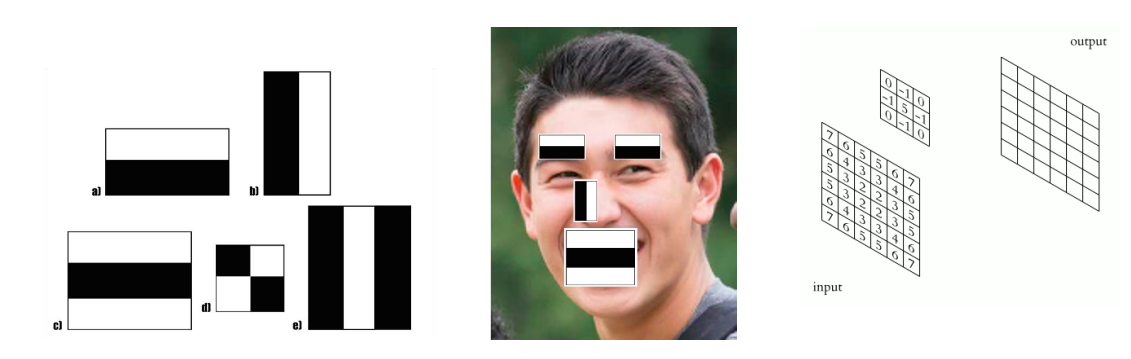
\includegraphics[width=1\linewidth]{haar_cascade.png}
    \caption{Minh họa kết quả phát hiện khuôn mặt bằng Haar Cascade}
    \label{fig:haar_detection}
\end{figure}
\subsection{Nhận diện khuôn mặt bằng LBPH}

LBPH (Local Binary Patterns Histograms) là phương pháp nhận diện khuôn mặt dựa trên mô tả kết cấu cục bộ \cite{lbph2006}. Thay vì học đặc trưng sâu, LBPH mã hóa mối quan hệ sáng/tối giữa một pixel trung tâm và các pixel lân cận. Điều này làm cho thuật toán nhẹ, dễ huấn luyện với số lượng mẫu nhỏ và phù hợp với thiết bị nhúng.

\subsubsection{Toán tử Local Binary Pattern}

Với một pixel trung tâm có cường độ $i_c$ và $P$ pixel lân cận có cường độ $i_p$, mã LBP được tính:

\begin{equation}
    LBP(x_c,y_c) = \sum_{p=0}^{P-1} s(i_p - i_c)2^p
\end{equation}

\begin{equation}
    s(u) =
    \begin{cases}
        1, & u \ge 0 \\
        0, & u < 0
    \end{cases}
\end{equation}

Kết quả là một số nhị phân mô tả mẫu kết cấu quanh pixel trung tâm. Ví dụ, vùng mắt, mũi, miệng và viền mặt tạo ra các mẫu sáng/tối khác nhau. Khi tính LBP cho toàn bộ ROI khuôn mặt, ta thu được bản đồ kết cấu cục bộ của khuôn mặt đó.

\subsubsection{Histogram theo lưới}

Nếu chỉ gom histogram trên toàn ảnh, thông tin vị trí của đặc trưng sẽ bị mất. Vì vậy LBPH chia khuôn mặt thành các ô lưới, tính histogram LBP cho từng ô, sau đó nối các histogram lại thành vector đặc trưng cuối cùng. Trong hệ thống, ROI khuôn mặt được resize về $100\times100$ pixel và mô hình LBPH được huấn luyện với các tham số ở Bảng \ref{tab:lbph_params}.

\begin{table}[H]
\centering
\caption{Tham số LBPH sử dụng khi huấn luyện}
\label{tab:lbph_params}
\begin{tabular}{|l|c|p{7.5cm}|}
\hline
\textbf{Tham số} & \textbf{Giá trị} & \textbf{Ý nghĩa} \\
\hline
\texttt{radius} & 1 & Bán kính vùng lân cận quanh pixel trung tâm. \\
\hline
\texttt{neighbors} & 8 & Số điểm lân cận dùng để tạo mã LBP. \\
\hline
\texttt{grid\_x} & 8 & Số ô chia theo chiều ngang khuôn mặt. \\
\hline
\texttt{grid\_y} & 8 & Số ô chia theo chiều dọc khuôn mặt. \\
\hline
Kích thước ROI & $100\times100$ & Kích thước chuẩn hóa trước khi huấn luyện và dự đoán. \\
\hline
\end{tabular}
\end{table}

Trong OpenCV, bộ nhận diện LBPH trả về hai giá trị \cite{opencv}:

\begin{itemize}
    \item \textbf{label}: mã định danh của người có histogram gần nhất với mẫu đầu vào.
    \item \textbf{confidence}: khoảng cách LBPH giữa mẫu đầu vào và mẫu đã học. Đây là khoảng cách, không phải xác suất; giá trị càng nhỏ thì khuôn mặt càng giống dữ liệu huấn luyện.
\end{itemize}

Hệ thống dùng ngưỡng \texttt{RECOGNITION\_THRESH = 150.0}. Nếu khoảng cách LBPH $d$ lớn hơn hoặc bằng ngưỡng này, khuôn mặt được xem là \texttt{Unknown}. Nếu nhỏ hơn ngưỡng, \texttt{label} được ánh xạ sang tên người dùng thông qua file JSON đi kèm mô hình.

\subsubsection{Chuẩn hóa độ tin cậy cho fuzzy logic}

Vì \texttt{confidence} của OpenCV LBPH là khoảng cách, hệ thống cần chuyển nó thành giá trị ``độ tin cậy mô hình'' theo hướng càng lớn càng đáng tin. Công thức được sử dụng:

\begin{equation}
    C_{raw} = \max\left(0,\ 100 - \frac{70d}{150}\right)
\end{equation}

Trong đó $d$ là khoảng cách LBPH. Khi $d=0$, mô hình có độ tin cậy rất cao. Khi $d=150$, giá trị còn khoảng 30, nằm gần vùng rủi ro cao trong bộ fuzzy. Trong bộ điều khiển fuzzy, biến \texttt{model\_confidence} được khai báo trên miền $[0,85]$; các giá trị cao hơn biên này được xem như mức HIGH tối đa.

\begin{figure}[H]
    \centering
    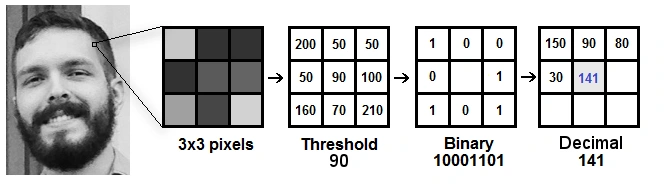
\includegraphics[width=1\linewidth]{lbph.png}
    \caption{Minh họa đặc trưng LBPH theo các vùng lưới của khuôn mặt}
    \label{fig:lbph_grid_todo}
\end{figure}

\subsection{Các đặc trưng chất lượng ảnh}

Kết quả nhận diện khuôn mặt phụ thuộc mạnh vào chất lượng ảnh. Một người đúng danh tính nhưng đứng trong ánh sáng quá yếu, quay mặt lệch hoặc frame bị mờ có thể làm tăng khoảng cách LBPH. Nếu hệ thống chỉ dùng ngưỡng nhận diện cứng, quyết định mở khóa có thể quá đơn giản. Vì vậy, hệ thống đo thêm ba đặc trưng chất lượng ảnh: độ sáng khuôn mặt, góc lệch tương đối và độ mờ.

\subsubsection{Độ sáng khuôn mặt}

Độ sáng được tính bằng giá trị trung bình của ảnh grayscale trong vùng khuôn mặt:

\begin{equation}
    I = \frac{1}{N}\sum_{p \in ROI} p
\end{equation}

Trong đó $ROI$ là vùng ảnh khuôn mặt và $N$ là số pixel trong vùng đó. Giá trị $I$ nằm trong khoảng $[0,255]$. Khi $I$ quá thấp, ảnh thiếu sáng và các chi tiết như mắt, mũi, miệng khó phân biệt. Khi $I$ quá cao, ảnh có thể bị cháy sáng, làm mất kết cấu cục bộ cần cho LBPH.

Trong bước đăng ký, hệ thống chỉ nhận mẫu nếu $35 \le I \le 230$. Khoảng này không đảm bảo ảnh hoàn hảo, nhưng loại bỏ được các frame quá tối hoặc quá sáng.

\subsubsection{Góc lệch tương đối}

Hệ thống không dùng mô hình head-pose estimation đầy đủ. Thay vào đó, góc lệch tương đối được ước lượng nhẹ bằng độ bất đối xứng sáng giữa nửa trái và nửa phải của ROI khuôn mặt:

\begin{equation}
    A = \frac{|\mu_L - \mu_R|}{\mu_L + \mu_R}
\end{equation}

\begin{equation}
    \theta = \min(180A,\ 90)
\end{equation}

Trong đó $\mu_L$ và $\mu_R$ là độ sáng trung bình của hai nửa khuôn mặt. Khi người dùng nhìn thẳng vào camera, hai nửa mặt thường có phân bố sáng tương đối cân bằng nên $A$ nhỏ. Khi mặt quay nghiêng hoặc một nửa mặt bị tối mạnh, $A$ tăng và góc ước lượng $\theta$ lớn hơn.

Cách ước lượng này có chi phí thấp và đủ dùng như một tín hiệu chất lượng cho fuzzy logic. Tuy nhiên, nó không phải là góc yaw hình học chính xác. Các trường hợp ánh sáng chiếu lệch mạnh có thể làm hệ thống đánh giá mặt đang bị lệch dù người dùng vẫn nhìn thẳng.

\subsubsection{Độ mờ khi đăng ký}

Khi đăng ký khuôn mặt, hệ thống dùng phương sai Laplacian để loại ảnh mờ. Laplacian phản ứng mạnh với biên và chi tiết cao tần. Nếu ảnh bị mờ, biên yếu đi và phương sai Laplacian giảm:

\begin{equation}
    B = Var(\nabla^2 ROI)
\end{equation}

Nếu $B < 20$, frame bị xem là quá mờ và không được lưu làm mẫu huấn luyện. Việc lọc mẫu mờ trong giai đoạn đăng ký rất quan trọng, vì dữ liệu đăng ký kém sẽ làm LBPH học histogram không đại diện, từ đó tăng lỗi nhận diện trong giai đoạn vận hành.

\begin{table}[H]
\centering
\caption{Điều kiện lọc mẫu khi đăng ký khuôn mặt}
\label{tab:registration_quality}
\begin{tabular}{|l|c|p{7cm}|}
\hline
\textbf{Tiêu chí} & \textbf{Ngưỡng} & \textbf{Mục đích} \\
\hline
Số khuôn mặt & Đúng 1 & Tránh gán nhầm mẫu của người khác vào identity đang đăng ký. \\
\hline
Kích thước mặt & $\min(w,h) \ge 32$ & Loại khuôn mặt quá nhỏ hoặc đứng quá xa camera. \\
\hline
Độ sáng & $35 \le I \le 230$ & Loại frame quá tối hoặc quá sáng. \\
\hline
Góc lệch & $\theta \le 40^\circ$ & Ưu tiên mẫu nhìn tương đối thẳng vào camera. \\
\hline
Độ mờ & $B \ge 20$ & Loại frame nhòe, rung hoặc mất chi tiết. \\
\hline
Khoảng cách thời gian & $\ge 0.25$s & Tránh lưu quá nhiều frame gần như giống hệt nhau. \\
\hline
Khác biệt với mẫu trước & $\ge 1.5$ & Khuyến khích người dùng thay đổi nhẹ tư thế để tăng đa dạng dữ liệu. \\
\hline
\end{tabular}
\end{table}

Sau khi một mẫu được chấp nhận, ROI được resize về $100\times100$ và cân bằng histogram bằng \texttt{equalizeHist}. Bước cân bằng histogram giúp giảm ảnh hưởng của chênh lệch sáng nhẹ giữa các lần chụp.

\subsection{Fuzzy logic Mamdani}

Fuzzy logic cho phép biểu diễn các khái niệm không có ranh giới cứng như ``độ tin cậy cao'', ``ánh sáng bình thường'' hoặc ``góc mặt lệch'' \cite{zadeh1965}. Trong khóa cửa thông minh, cách tiếp cận này phù hợp hơn một luật ngưỡng đơn giản vì quyết định truy cập nên xét đồng thời nhiều yếu tố. Ví dụ, một khuôn mặt có LBPH tốt nhưng ánh sáng quá xấu có thể cần rủi ro trung bình thay vì mở khóa ngay.

Hệ thống sử dụng bộ suy luận Mamdani \cite{mamdani1975} được hiện thực bằng pyfuzzylite \cite{fuzzylite}. Bộ điều khiển gồm bốn bước:

\begin{enumerate}
    \item \textbf{Fuzzification}: chuyển giá trị số thành mức thuộc về các tập mờ.
    \item \textbf{Rule evaluation}: đánh giá các luật IF--THEN bằng toán tử mờ.
    \item \textbf{Aggregation}: gom kết quả của nhiều luật thành một tập mờ đầu ra.
    \item \textbf{Defuzzification}: chuyển tập mờ đầu ra thành một giá trị rủi ro cụ thể.
\end{enumerate}

\subsubsection{Hàm thành viên Gaussian}

Các tập mờ trong hệ thống dùng hàm thành viên Gaussian:

\begin{equation}
    \mu(x) = \exp\left(-\frac{(x-c)^2}{2\sigma^2}\right)
\end{equation}

Trong đó $c$ là tâm của tập mờ và $\sigma$ là độ lệch chuẩn. Hàm Gaussian tạo ra biên chuyển mềm giữa các mức LOW, MEDIUM, HIGH thay vì thay đổi đột ngột tại một ngưỡng duy nhất.

\begin{table}[H]
\centering
\caption{Biến đầu vào của bộ fuzzy}
\label{tab:fuzzy_inputs}
\begin{tabular}{|l|c|l|}
\hline
\textbf{Biến} & \textbf{Miền giá trị} & \textbf{Tập mờ Gaussian $(c,\sigma)$} \\
\hline
Độ tin cậy mô hình & 0--85 & LOW $(0,17)$, MEDIUM $(42.5,10)$, HIGH $(85,17)$ \\
\hline
Độ sáng khuôn mặt & 0--255 & DARK $(0,40)$, NORMAL $(128,45)$, BRIGHT $(255,40)$ \\
\hline
Góc lệch khuôn mặt & 0--90 & FRONTAL $(0,20)$, MARGINAL $(90,40)$ \\
\hline
\end{tabular}
\end{table}

Biến đầu ra là \textbf{security risk} trong khoảng $[0,1]$. Giá trị càng gần 0 thì hệ thống càng an toàn để mở khóa; giá trị càng gần 1 thì rủi ro càng cao.

\begin{table}[H]
\centering
\caption{Biến đầu ra của bộ fuzzy}
\label{tab:fuzzy_output}
\begin{tabular}{|l|c|l|}
\hline
\textbf{Biến} & \textbf{Miền giá trị} & \textbf{Tập mờ Gaussian $(c,\sigma)$} \\
\hline
Security risk & 0--1 & MINIMUM $(0,0.1)$, AVERAGE $(0.5,0.1)$, MAXIMUM $(1,0.08)$ \\
\hline
\end{tabular}
\end{table}

Các hàm thành viên trong Bảng \ref{tab:fuzzy_inputs} và Bảng \ref{tab:fuzzy_output} được minh họa ở Hình \ref{fig:fuzzy_membership_todo}. Phần giao nhau giữa các đường cong cho phép một frame kích hoạt đồng thời nhiều luật với các mức độ khác nhau, nhờ đó quyết định không bị phụ thuộc vào một ngưỡng cứng duy nhất.

\begin{figure}[H]
    \centering
    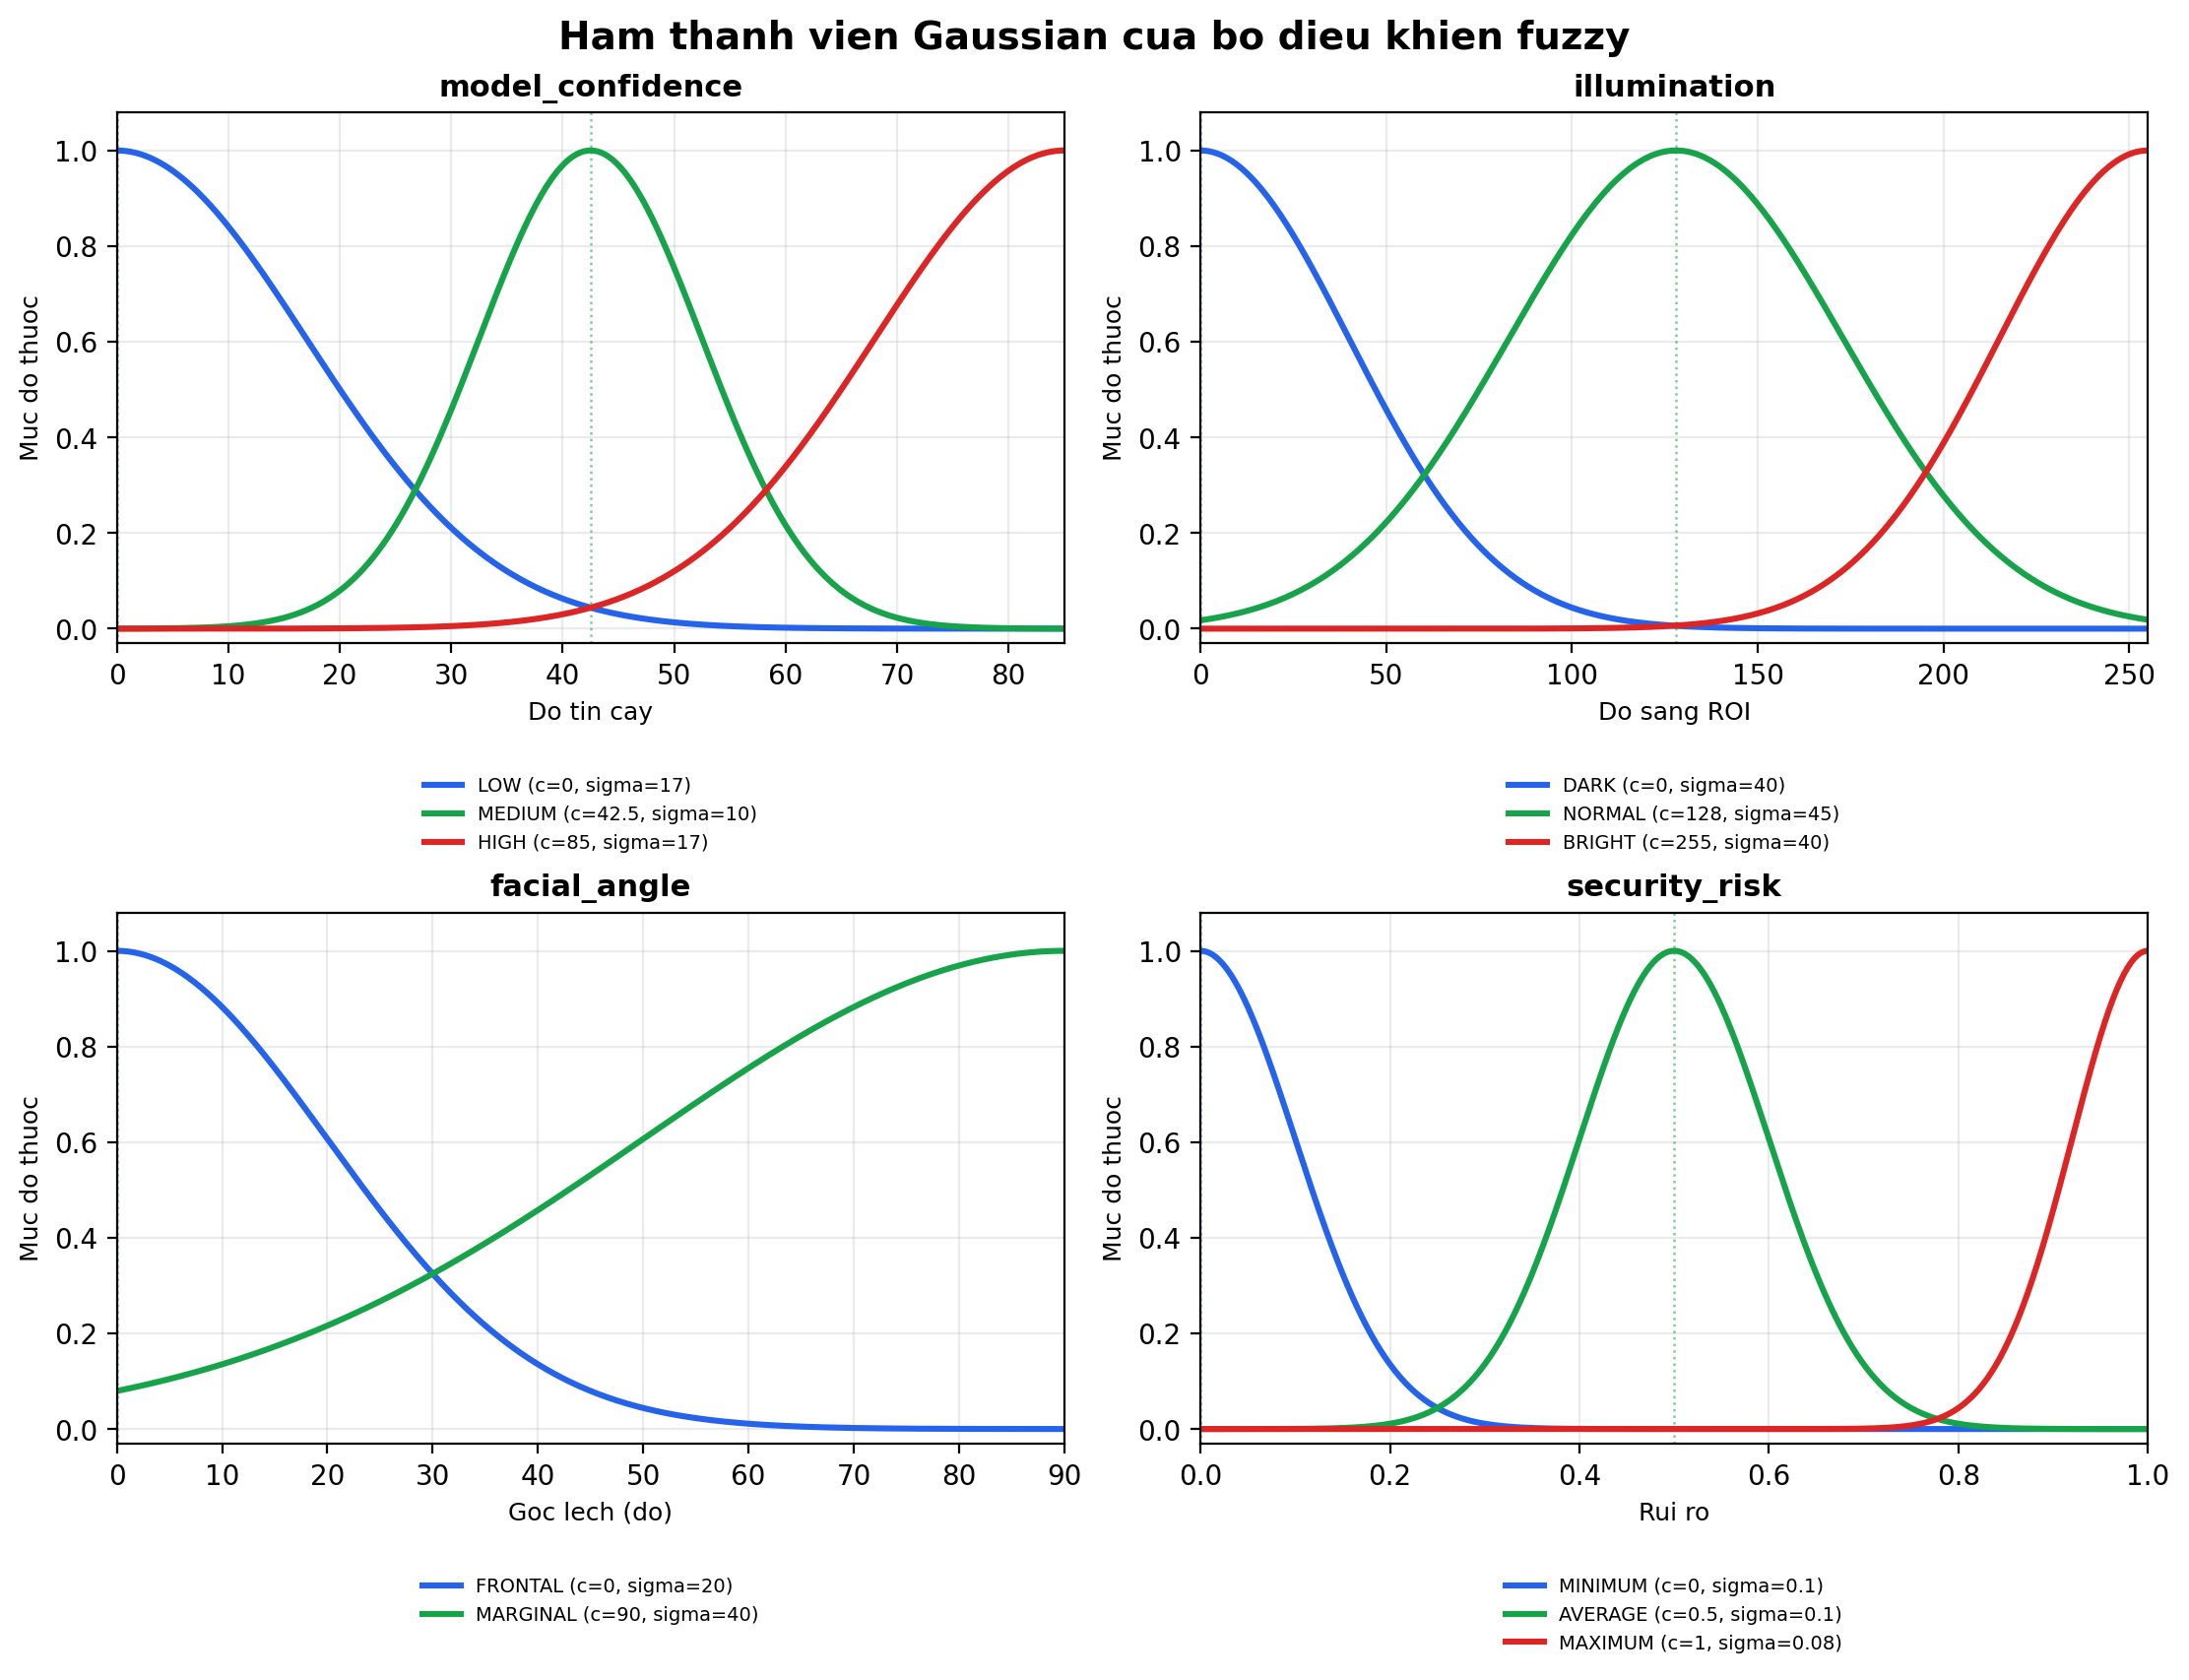
\includegraphics[width=\linewidth]{fuzzy_full.png}
    \caption{Minh họa các hàm thành viên của bộ điều khiển fuzzy}
    \label{fig:fuzzy_membership_todo}
\end{figure}

\subsubsection{Toán tử Mamdani và giải mờ}

Trong bộ điều khiển, phép AND được cài bằng toán tử Minimum, phép OR bằng Maximum, phép suy diễn bằng Minimum và phép tổng hợp các luật bằng Maximum. Sau khi tổng hợp, hệ thống dùng phương pháp centroid để giải mờ:

\begin{equation}
    r = \frac{\int z\mu_{out}(z)\,dz}{\int \mu_{out}(z)\,dz}
\end{equation}

Trong đó $r$ là giá trị rủi ro rõ cuối cùng, còn $\mu_{out}(z)$ là hàm thành viên đầu ra sau khi tất cả luật được kích hoạt. Trong code, centroid được lấy mẫu với độ phân giải 200 điểm, đủ cho miền đầu ra nhỏ $[0,1]$.

\subsubsection{Nhóm luật quyết định}

Bộ điều khiển sử dụng 13 luật. Các luật được thiết kế theo nguyên tắc fail-safe: khi danh tính không đáng tin hoặc điều kiện ảnh xấu, rủi ro phải tăng; hệ thống chỉ mở khóa khi độ tin cậy cao, ánh sáng bình thường và khuôn mặt nhìn thẳng.

\begin{table}[H]
\centering
\caption{Tóm tắt nhóm luật fuzzy}
\label{tab:fuzzy_rule_groups}
\begin{tabular}{|p{3.2cm}|p{3.4cm}|p{2.8cm}|p{2.5cm}|}
\hline
\textbf{Model confidence} & \textbf{Illumination} & \textbf{Facial angle} & \textbf{Risk} \\
\hline
LOW & Bất kỳ & Bất kỳ & MAXIMUM \\
\hline
HIGH & NORMAL & FRONTAL & MINIMUM \\
\hline
HIGH & NORMAL & MARGINAL & AVERAGE \\
\hline
HIGH & DARK hoặc BRIGHT & Bất kỳ & AVERAGE \\
\hline
MEDIUM & NORMAL & FRONTAL & AVERAGE \\
\hline
MEDIUM & NORMAL & MARGINAL & MAXIMUM \\
\hline
MEDIUM & DARK & Bất kỳ & MAXIMUM \\
\hline
MEDIUM & BRIGHT & FRONTAL hoặc MARGINAL & AVERAGE \\
\hline
\end{tabular}
\end{table}

Nếu không có khuôn mặt trong frame, hệ thống không chạy mở khóa mà trả về rủi ro 1.0 và hành động \texttt{deny}. Nếu thư viện pyfuzzylite không khả dụng, backend có fallback logic tĩnh để hệ thống vẫn chạy theo hướng an toàn: độ tin cậy thấp hoặc điều kiện ảnh kém luôn dẫn tới rủi ro cao.

\subsubsection{Ánh xạ rủi ro thành hành động}

Giá trị crisp cuối cùng được ánh xạ thành hành động như Bảng \ref{tab:risk_action_map}. Hành động \texttt{otp} được hiểu là trạng thái cần xác thực bổ sung; trong bản hiện thực hiện tại, luồng keypad đóng vai trò kênh xác thực thứ hai độc lập.

\begin{table}[H]
\centering
\caption{Ánh xạ rủi ro thành hành động}
\label{tab:risk_action_map}
\begin{tabular}{|c|l|l|}
\hline
\textbf{Khoảng rủi ro} & \textbf{Hành động} & \textbf{Ý nghĩa} \\
\hline
$r < 0.30$ & \texttt{unlock} & Mở khóa bằng servo. \\
\hline
$0.30 \le r < 0.60$ & \texttt{otp} & Cần xác thực bổ sung. \\
\hline
$0.60 \le r < 0.85$ & \texttt{deny} & Từ chối truy cập và ghi nhận sự kiện. \\
\hline
$r \ge 0.85$ & \texttt{lockout} & Rủi ro rất cao, khóa tạm thời hoặc cảnh báo. \\
\hline
\end{tabular}
\end{table}

\subsection{Xác thực bằng keypad và mã PIN}

Ngoài nhận diện khuôn mặt, hệ thống có keypad 4x4 để nhập mã PIN 6 chữ số. Đây là một kênh xác thực khác với nhận diện khuôn mặt, giúp người dùng vẫn có thể mở khóa trong trường hợp camera, ánh sáng hoặc mô hình nhận diện không hoạt động tốt.

Về mặt bảo mật, hệ thống không so sánh trực tiếp chuỗi PIN dạng rõ. PIN được băm bằng SHA-256:

\begin{equation}
    H = SHA256(PIN)
\end{equation}

Khi người dùng nhập PIN, hệ thống băm chuỗi vừa nhập và so sánh với hash đang lưu trong bộ nhớ. Hàm băm một chiều giúp tránh việc lưu trực tiếp mật khẩu dạng rõ trong biến trạng thái. Mã PIN mới cũng phải có đúng 6 chữ số và chỉ được cập nhật khi người dùng nhập đúng PIN hiện tại.

Để hạn chế thử sai liên tục, keypad dùng cơ chế lockout. Sau 5 lần nhập sai, keypad bị khóa trong 30 giây. Ngoài ra, nếu người dùng bắt đầu nhập nhưng dừng quá lâu, buffer nhập PIN được xóa sau 10 giây. Các cơ chế này làm giảm nguy cơ brute-force đơn giản trên keypad vật lý.

\subsection{FastAPI, REST và cơ chế polling}

FastAPI là framework Python dùng để xây dựng API bất đồng bộ, có kiểu dữ liệu rõ ràng và tự sinh tài liệu OpenAPI \cite{fastapi}. Trong hệ thống, FastAPI quản lý vòng đời backend, khởi động camera worker khi ứng dụng start và dừng worker khi shutdown. Backend cũng cung cấp các endpoint để frontend đọc frame mới nhất, xem trạng thái camera, đăng ký khuôn mặt và đổi mật khẩu keypad.

Luồng camera không được truyền bằng WebSocket hay RTSP. Thay vào đó, worker xử lý frame trong background thread, encode frame đã vẽ kết quả thành JPEG base64 và lưu vào cache mới nhất. Frontend gọi \texttt{/api/v1/camera/frame} theo chu kỳ ngắn để lấy frame và metadata. Cơ chế này gọi là polling.

\begin{table}[H]
\centering
\caption{Các endpoint REST chính liên quan đến cơ sở lý thuyết hệ thống}
\label{tab:rest_theory_endpoints}
\begin{tabular}{|l|l|p{6.2cm}|}
\hline
\textbf{Phương thức} & \textbf{Endpoint} & \textbf{Vai trò} \\
\hline
GET & \texttt{/api/v1/camera/frame} & Trả về frame JPEG base64, danh sách khuôn mặt, kết quả fuzzy và trạng thái đăng ký. \\
\hline
GET & \texttt{/api/v1/camera/history} & Trả về lịch sử gần đây của nhận diện và quyết định truy cập. \\
\hline
POST & \texttt{/api/v1/register/start} & Bắt đầu phiên thu mẫu khuôn mặt cho một người dùng. \\
\hline
POST & \texttt{/api/v1/register/cancel} & Hủy phiên đăng ký đang chạy. \\
\hline
POST & \texttt{/api/v1/keypad/password} & Đổi mã PIN keypad sau khi xác thực PIN hiện tại. \\
\hline
GET & \texttt{/api/v1/keypad/status} & Trả về trạng thái keypad, số lần sai và thời gian lockout còn lại. \\
\hline
\end{tabular}
\end{table}

Polling có ưu điểm là đơn giản, dễ debug, dễ triển khai trong demo cục bộ và tương thích tốt với HTTP thông thường. Nhược điểm là frontend vẫn gửi request định kỳ kể cả khi frame không đổi. Trong hệ thống này, chu kỳ polling khoảng 250 ms là phù hợp vì frame đã được xử lý ở backend và kích thước ảnh JPEG base64 không quá lớn.

\subsection{Frontend Next.js}

Next.js là framework React hỗ trợ xây dựng giao diện web hiện đại \cite{nextjs}. Frontend trong đề tài đóng vai trò dashboard quan sát và điều khiển. Nó không truy cập camera trực tiếp, không chạy mô hình nhận diện và không điều khiển GPIO. Tất cả thao tác phần cứng và xử lý ảnh nằm ở backend; frontend chỉ gửi HTTP request và hiển thị dữ liệu nhận được.

Component hiển thị video gọi API theo chu kỳ, nhận \texttt{frame\_base64}, chuyển thành URL dạng \texttt{data:image/jpeg;base64,...} và hiển thị bằng thẻ \texttt{img}. Cùng với ảnh, frontend hiển thị số khuôn mặt, danh tính, khoảng cách LBPH, độ sáng, góc mặt, hành động fuzzy và phần trăm rủi ro. Cách hiển thị này giúp người vận hành quan sát được không chỉ kết quả cuối cùng, mà cả lý do hệ thống đưa ra quyết định.

Frontend cũng cung cấp form đăng ký khuôn mặt và form đổi mật khẩu keypad. Các form này kiểm tra dữ liệu cơ bản ở phía trình duyệt, ví dụ mã PIN phải gồm đúng 6 chữ số, sau đó gửi request đến FastAPI để xử lý chính thức.

\subsection{Nền tảng Raspberry Pi và ngoại vi}

Raspberry Pi đóng vai trò bộ điều khiển trung tâm của hệ thống \cite{raspberrypi}. Thiết bị vừa chạy backend Python, vừa đọc camera, vừa giao tiếp với keypad, OLED và servo. Các ngoại vi này giúp hệ thống hoạt động như một khóa cửa vật lý thay vì chỉ là demo nhận diện trên màn hình.

\subsubsection{Keypad ma trận 4x4}

Keypad 4x4 gồm 4 hàng và 4 cột. Về nguyên lý, mỗi phím là một công tắc nối một hàng với một cột. Để xác định phím được nhấn, hệ thống đặt các chân hàng làm output và các chân cột làm input với pull-down. Khi có cạnh rising ở một cột, callback ngắt được kích hoạt. Sau đó backend lần lượt kéo từng hàng lên mức HIGH để tìm giao điểm hàng--cột tương ứng với phím.

Cách dùng interrupt giúp giảm tải CPU so với việc polling keypad liên tục. Hệ thống cũng áp dụng debounce 250 ms để giảm hiện tượng một lần nhấn phím bị ghi nhận thành nhiều lần do rung tiếp điểm cơ khí.

\subsubsection{OLED SSD1306}

OLED SSD1306 kích thước 128x64 được dùng để hiển thị trạng thái hệ thống: màn hình chờ, nhập PIN, đăng ký khuôn mặt, mở khóa thành công, từ chối truy cập và lockout. Thư viện luma.oled được sử dụng để giao tiếp với màn hình \cite{lumaoled}. Backend render nội dung bằng Pillow rồi gửi buffer ảnh sang OLED qua bus SPI.

OLED rất quan trọng trong kịch bản khóa cửa vì người dùng đứng trước cửa không nhất thiết đang nhìn dashboard web. Các thông báo như số chữ số PIN đã nhập, số lần sai còn lại hoặc thời gian lockout cần được hiển thị trực tiếp trên thiết bị.

\subsubsection{Servo điều khiển chốt khóa}

Servo mô phỏng cơ cấu chốt khóa cửa. Servo được điều khiển bằng PWM 50 Hz. Trong hệ thống, duty cycle khoảng 7.5 dùng cho trạng thái mở khóa và khoảng 2.5 dùng cho trạng thái khóa. Sau khi servo quay đến vị trí mong muốn, duty cycle được đưa về 0 để giảm rung, giảm tiếng kêu và tiết kiệm năng lượng.

Servo nên dùng nguồn 5V ngoài thay vì lấy trực tiếp từ chân 5V của Raspberry Pi. Dòng khởi động của servo có thể làm sụt áp và khiến Pi reset. Tuy nhiên, nguồn servo và Raspberry Pi phải nối chung GND để tín hiệu PWM có cùng mức tham chiếu.

\begin{table}[H]
\centering
\caption{Các ngoại vi chính của hệ thống}
\label{tab:hardware_theory}
\begin{tabular}{|l|l|p{6.7cm}|}
\hline
\textbf{Thiết bị} & \textbf{Giao tiếp} & \textbf{Vai trò} \\
\hline
Camera USB/V4L2 & Video capture & Cung cấp frame đầu vào cho pipeline Haar, LBPH và fuzzy. \\
\hline
Keypad 4x4 & GPIO input/output & Nhập mã PIN 6 chữ số và xác thực dự phòng. \\
\hline
OLED SSD1306 & SPI & Hiển thị trạng thái trực tiếp trên thiết bị. \\
\hline
Servo & PWM 50 Hz & Mô phỏng cơ cấu mở/khóa chốt cửa. \\
\hline
\end{tabular}
\end{table}

\section{Thiết kế hệ thống}

\subsection{Kiến trúc tổng quan}

SmartLock Fuzzy được thiết kế theo mô hình backend trung tâm. Backend sở hữu camera và phần cứng, còn frontend chỉ đóng vai trò giao diện quan sát/điều khiển qua HTTP API với FastAPI và Next.js \cite{fastapi,nextjs}.


\begin{figure}[H]
\centering
\resizebox{\textwidth}{!}{%
\begin{tikzpicture}[
    >=Stealth,
    font=\small,
    block/.style={
        draw,
        rounded corners,
        minimum width=3.3cm,
        minimum height=0.9cm,
        align=center
    },
    hw/.style={
        draw,
        rounded corners,
        minimum width=3.0cm,
        minimum height=0.85cm,
        align=center
    },
    data/.style={thick, -{Stealth}},
    http/.style={thick, {Stealth}-{Stealth}},
    ctrl/.style={thick, dashed, -{Stealth}},
    lab/.style={
        font=\scriptsize,
        fill=white,
        inner sep=1.5pt
    }
]

% ---------------- Nodes ----------------
\node[hw]    (cam)          at (0,  1.4) {Camera\\\texttt{/dev/video0}};
\node[hw]    (hardware)     at (0, -1.4) {Keypad/OLED/Servo\\GPIO + SPI + PWM};

\node[block] (worker)       at (4.2, 0) {\texttt{LocalCameraWorker}\\vòng lặp xử lý};

\node[block] (api)          at (8.5, 1.4) {FastAPI\\REST endpoints};
\node[block] (front)        at (12.7, 1.4) {Next.js Dashboard\\polling HTTP};

\node[block] (vision)       at (8.5, -0.4) {OpenCV\\Haar + LBPH};
\node[block] (fuzzy)        at (8.5, -2.2) {Fuzzy Controller\\Mamdani rules};

\node[block] (registration) at (4.2, -2.2) {Registration Manager\\thu mẫu + train LBPH};

% ---------------- Data flow ----------------
\draw[data] (cam.east) -- node[lab, above] {frame} (worker.west);

\draw[data] (worker.north east) -- node[lab, above] {latest frame/status} (api.west);
\draw[http] (api.east) -- node[lab, above] {GET/POST} (front.west);

\draw[data] (worker.east) -- node[lab, above] {frame} (vision.west);
\draw[data] (vision.south) -- node[lab, right] {detection} (fuzzy.north);

\draw[data] (worker.south) -- node[lab, right] {samples} (registration.north);

% ---------------- Hardware control ----------------
\draw[ctrl] (worker.south west) to[bend right=15]
    node[lab, left] {unlock/status} (hardware.east);

\draw[ctrl] (hardware.east) to[bend right=15]
    node[lab, below] {keypad event} (worker.west);

\end{tikzpicture}
}
\caption{Kiến trúc tổng quan của hệ thống SmartLock Fuzzy}
\label{fig:system_architecture}
\end{figure}

Các thành phần chính:

\begin{itemize}
    \item \textbf{Backend FastAPI}: quản lý vòng đời hệ thống, API và worker camera.
    \item \textbf{Camera worker}: xử lý frame, nhận diện, đánh giá fuzzy và cập nhật trạng thái mới nhất.
    \item \textbf{Service xử lý ảnh}: đóng gói Haar Cascade, LBPH và các phép đo chất lượng khuôn mặt.
    \item \textbf{Service fuzzy}: ánh xạ kết quả nhận diện thành quyết định truy cập.
    \item \textbf{Service phần cứng}: điều khiển keypad, OLED và servo.
    \item \textbf{Frontend}: dashboard web để quan sát camera, đăng ký người dùng và đổi mật khẩu.
\end{itemize}

\subsection{Luồng xử lý camera}

Mỗi frame đi qua các bước sau:

\begin{enumerate}
    \item Đọc frame từ camera bằng OpenCV \cite{opencv}.
    \item Lật ảnh nếu biến môi trường \texttt{CAMERA\_FLIP} được bật.
    \item Phát hiện khuôn mặt bằng Haar Cascade \cite{viola2001}.
    \item Nếu có nhiều khuôn mặt, giữ khuôn mặt có bounding box lớn nhất.
    \item Nhận diện bằng LBPH nếu model đã được nạp \cite{lbph2006}.
    \item Tính độ sáng ROI và góc lệch tương đối.
    \item Đưa detection đầu tiên vào bộ fuzzy để tính \texttt{security\_risk}.
    \item Nếu hành động là \texttt{unlock} và keypad không hoạt động, kích hoạt servo mở khóa.
    \item Xử lý đăng ký khuôn mặt nếu đang có session đăng ký.
    \item Vẽ overlay, mã hóa JPEG base64 và cập nhật cache API.
\end{enumerate}

\begin{figure}[H]
\centering
\resizebox{\textwidth}{!}{%
\begin{tikzpicture}[
    >=Stealth,
    node distance=0.85cm,
    step/.style={draw, rounded corners, minimum width=3.0cm, minimum height=0.8cm, align=center, font=\small},
    arrow/.style={thick, -{Stealth}}
]
    \node[step] (read) {Đọc frame};
    \node[step, right=of read] (detect) {Haar detect};
    \node[step, right=of detect] (lbph) {LBPH recognize};
    \node[step, right=of lbph] (quality) {Đo sáng/góc};
    \node[step, below=of quality] (fuzzy) {Fuzzy risk};
    \node[step, left=of fuzzy] (action) {Quyết định};
    \node[step, left=of action] (encode) {Overlay + JPEG};
    \node[step, left=of encode] (api) {API cache};

    \draw[arrow] (read) -- (detect);
    \draw[arrow] (detect) -- (lbph);
    \draw[arrow] (lbph) -- (quality);
    \draw[arrow] (quality) -- (fuzzy);
    \draw[arrow] (fuzzy) -- (action);
    \draw[arrow] (action) -- (encode);
    \draw[arrow] (encode) -- (api);
\end{tikzpicture}
}
\caption{Pipeline xử lý một frame camera}
\label{fig:camera_pipeline}
\end{figure}

\subsection{Thiết kế API}

Backend cung cấp các endpoint chính sau:

\begin{table}[H]
\centering
\caption{Danh sách endpoint của hệ thống}
\label{tab:api_endpoints}
\begin{tabularx}{\textwidth}{|l|l|X|}
\hline
\textbf{Method} & \textbf{Endpoint} & \textbf{Chức năng} \\
\hline
GET & \texttt{/health} & Kiểm tra backend còn hoạt động. \\
\hline
GET & \texttt{/camera/status} & Trạng thái camera worker, đăng ký và phần cứng. \\
\hline
GET & \texttt{/api/v1/camera/frame} & Metadata và frame JPEG base64 mới nhất. \\
\hline
GET & \texttt{/api/v1/camera/latest} & Metadata mới nhất, không kèm frame base64. \\
\hline
GET & \texttt{/api/v1/camera/history} & Lịch sử kết quả gần nhất. \\
\hline
POST & \texttt{/api/v1/register/start} & Bắt đầu thu mẫu đăng ký khuôn mặt. \\
\hline
POST & \texttt{/api/v1/register/cancel} & Hủy session đăng ký hiện tại. \\
\hline
GET & \texttt{/api/v1/register/status} & Lấy tiến trình đăng ký. \\
\hline
POST & \texttt{/api/v1/keypad/password} & Đổi mã PIN 6 chữ số. \\
\hline
GET & \texttt{/api/v1/keypad/status} & Lấy trạng thái keypad và lockout. \\
\hline
\end{tabularx}
\end{table}

Cache camera mới nhất được lưu trong module router và bảo vệ bằng \texttt{threading.Lock}. Cách này đơn giản, đủ dùng cho một backend cục bộ phục vụ dashboard.

\subsection{Thiết kế fuzzy decision}

Bộ fuzzy nhận detection đầu tiên. Nếu không có detection, hệ thống trả về \texttt{deny}. Nếu danh tính là \texttt{Unknown}, độ tin cậy mô hình được đặt bằng 0. Với người nhận diện được, khoảng cách LBPH được scale thành \texttt{model\_confidence}. Bộ fuzzy dùng 13 luật theo hướng Mamdani \cite{mamdani1975}:

\begin{itemize}
    \item LOW confidence luôn dẫn tới MAXIMUM risk.
    \item HIGH confidence, ánh sáng NORMAL và mặt FRONTAL dẫn tới MINIMUM risk.
    \item HIGH confidence nhưng ánh sáng/góc không tối ưu dẫn tới AVERAGE risk.
    \item MEDIUM confidence chỉ được xem là AVERAGE risk trong một số điều kiện thuận lợi; các điều kiện xấu tăng lên MAXIMUM risk.
\end{itemize}

Khi thư viện fuzzy không khả dụng, \texttt{services/fuzzy\_logic.py} có fallback logic tĩnh để backend không bị dừng. Fallback vẫn giữ nguyên tinh thần fail-safe: thiếu tin cậy thì rủi ro cao.

\subsection{Thiết kế đăng ký khuôn mặt}

Đăng ký khuôn mặt là một session có trạng thái. Người dùng nhập tên trên dashboard, backend tạo thư mục tương ứng trong \texttt{registered\_faces/}. Mỗi frame được kiểm tra chất lượng trước khi lưu:

\begin{itemize}
    \item Chỉ chấp nhận đúng một khuôn mặt.
    \item Kích thước khuôn mặt đủ lớn.
    \item Độ sáng trong khoảng an toàn.
    \item Góc mặt không vượt ngưỡng.
    \item Ảnh không quá mờ.
    \item Mẫu mới phải khác mẫu trước đó đủ lớn để tránh lưu các frame trùng lặp.
\end{itemize}

Khi đủ số mẫu, backend huấn luyện lại LBPH, ghi file XML và JSON label map, sau đó reload recognizer mà không cần khởi động lại server.

\subsection{Thiết kế phần cứng}

Bảng sau mô tả mapping GPIO mặc định:

\begin{table}[H]
\centering
\caption{Kết nối phần cứng Raspberry Pi}
\label{tab:hardware_pins}
\begin{tabular}{|l|l|l|}
\hline
\textbf{Thiết bị} & \textbf{Chức năng} & \textbf{GPIO BCM} \\
\hline
Keypad 4x4 & Row 1--4 & 17, 27, 22, 5 \\
\hline
Keypad 4x4 & Col 1--4 & 6, 13, 19, 26 \\
\hline
Servo & PWM signal & 18 \\
\hline
OLED SSD1306 SPI & DC, RST & 24, 25 \\
\hline
OLED SSD1306 SPI & MOSI, SCLK, CE0 & 10, 11, 8 \\
\hline
\end{tabular}
\end{table}

\begin{figure}[H]
\centering
\resizebox{\textwidth}{!}{%
\begin{tikzpicture}[
    >=Stealth,
    font=\small,
    pi/.style={draw, rounded corners, fill=green!8, minimum width=4.0cm, minimum height=5.8cm, align=center},
    dev/.style={draw, rounded corners, fill=blue!7, minimum width=3.6cm, minimum height=1.0cm, align=center},
    power/.style={draw, rounded corners, fill=red!7, minimum width=3.6cm, minimum height=1.0cm, align=center},
    wire/.style={thick, -{Stealth}},
    pwr/.style={thick, red!70!black, -{Stealth}},
    gnd/.style={thick, black!75, -{Stealth}},
    sig/.style={thick, blue!70!black, -{Stealth}},
    note/.style={font=\scriptsize, align=center, fill=white, inner sep=1pt}
]

\node[pi] (pi) at (0,0) {\textbf{Raspberry Pi 4B}\\[0.2cm]
\begin{tabular}{ll}
GPIO17 & Keypad R1\\
GPIO27 & Keypad R2\\
GPIO22 & Keypad R3\\
GPIO5  & Keypad R4\\
GPIO6  & Keypad C1\\
GPIO13 & Keypad C2\\
GPIO19 & Keypad C3\\
GPIO26 & Keypad C4\\
GPIO18 & Servo PWM\\
GPIO10 & OLED MOSI\\
GPIO11 & OLED SCLK\\
GPIO8  & OLED CS\\
GPIO24 & OLED DC\\
GPIO25 & OLED RST
\end{tabular}};

\node[dev] (cam) at (-5.6,2.4) {USB Camera\\\texttt{/dev/video0}};
\node[dev] (keypad) at (5.8,2.2) {Keypad 4x4\\R1--R4, C1--C4};
\node[dev] (oled) at (5.8,0.0) {OLED SSD1306 SPI\\VCC, GND, SCLK, MOSI, RST, DC, CS};
\node[dev] (servo) at (5.8,-2.2) {RC Servo\\Signal, 5V, GND};
\node[power] (supply) at (-5.6,-2.2) {Nguồn 5V ngoài\\cho servo};

\draw[wire] (cam.east) -- node[note, above] {USB} (pi.west);
\draw[sig] (pi.east) -- node[note, above] {8 GPIO matrix} (keypad.west);
\draw[sig] (pi.east) -- node[note, above] {SPI + DC/RST} (oled.west);
\draw[sig] (pi.east) -- node[note, above] {GPIO18 PWM} (servo.west);
\draw[pwr] (supply.east) -- node[note, below] {5V} (servo.west);
\draw[gnd] (supply.north east) to[bend left=18] node[note, above] {GND chung} (pi.south west);
\draw[gnd] (pi.south east) to[bend right=18] node[note, below] {GND} (servo.south west);

\end{tikzpicture}
}
\caption{Sơ đồ kết nối phần cứng của hệ thống SmartLock Fuzzy}
\label{fig:hardware_schematic}
\end{figure}

Keypad sử dụng interrupt trên các cột để tránh polling liên tục. Servo được điều khiển bằng PWM, sau đó duty cycle được đưa về 0 để giảm rung. OLED được render bằng Pillow trước khi gửi qua SPI qua thư viện luma.oled \cite{lumaoled}.

\subsection{Thiết kế frontend}

Frontend Next.js gồm ba thành phần chính:

\begin{itemize}
    \item \texttt{Header}: tiêu đề và trạng thái dashboard.
    \item \texttt{LiveVideoStream}: polling frame, hiển thị camera, thông tin nhận diện, fuzzy risk và form đăng ký.
    \item \texttt{PasswordChange}: đổi mật khẩu keypad, kiểm tra độ dài 6 chữ số và gửi API.
\end{itemize}

Frontend đọc biến môi trường \texttt{NEXT\_PUBLIC\_API\_URL}, mặc định là \texttt{http://localhost:8000}. Dashboard polling frame mỗi 250 ms, phù hợp cho demo live view cục bộ.

\section{Hiện thực hệ thống}

Chương này mô tả chi tiết phần hiện thực của SmartLock Fuzzy dựa trên mã nguồn hiện có trong repository. Khác với chương thiết kế, nội dung bên dưới tập trung vào cách các module được cài đặt, cách dữ liệu đi qua từng lớp, các biến môi trường, cấu trúc JSON, cơ chế đồng bộ thread và các ngưỡng được dùng trong code.

\subsection{Cấu trúc hiện thực tổng quát}

Hệ thống được chia thành ba khối hiện thực chính:

\begin{itemize}
    \item \textbf{Backend Python}: FastAPI, camera worker, xử lý ảnh OpenCV, fuzzy logic, đăng ký khuôn mặt và phần cứng.
    \item \textbf{Frontend Next.js}: dashboard web để xem camera, trạng thái fuzzy, đăng ký khuôn mặt và đổi mã PIN.
    \item \textbf{Script hỗ trợ}: huấn luyện, benchmark, đánh giá detector và kiểm tra phần cứng.
\end{itemize}

Các module backend quan trọng được đặt dưới thư mục \texttt{backend/}. Trong đó, \texttt{main.py} là entrypoint của API, \texttt{services/local\_camera.py} điều phối luồng camera, \texttt{services/face\_detection.py} đóng gói Haar Cascade và LBPH, \texttt{services/registration.py} quản lý đăng ký khuôn mặt, \texttt{infra/fuzzy\_controller.py} hiện thực bộ fuzzy Mamdani, \texttt{services/hardware\_io.py} điều khiển keypad/servo và \texttt{services/oled\_display.py} điều khiển OLED.

\begin{table}[H]
\centering
\caption{Các file hiện thực chính của backend}
\label{tab:backend_implementation_files}
\begin{tabularx}{\textwidth}{|l|X|}
\hline
\textbf{File} & \textbf{Vai trò} \\
\hline
\texttt{backend/main.py} & Khởi tạo FastAPI, logging, CORS, lifespan và các endpoint cấp cao. \\
\hline
\texttt{backend/routers/get\_camera.py} & Lưu cache frame mới nhất, metadata, lịch sử nhận diện và endpoint đọc camera. \\
\hline
\texttt{backend/services/local\_camera.py} & Thread nền đọc camera, gọi nhận diện, fuzzy, đăng ký, OLED, servo và cập nhật API cache. \\
\hline
\texttt{backend/services/face\_detection.py} & Phát hiện mặt bằng Haar, nhận diện LBPH, đo illumination/facial angle và trích ROI đăng ký. \\
\hline
\texttt{backend/services/registration.py} & Thu mẫu khuôn mặt, lọc chất lượng, lưu ảnh mẫu và huấn luyện lại LBPH. \\
\hline
\texttt{backend/infra/fuzzy\_controller.py} & Xây dựng fuzzy engine bằng pyfuzzylite với 3 input, 1 output và 13 luật. \\
\hline
\texttt{backend/services/fuzzy\_logic.py} & Wrapper chuyển detection thành input fuzzy và fallback khi pyfuzzylite không khả dụng. \\
\hline
\texttt{backend/services/hardware\_io.py} & Điều khiển keypad interrupt-driven, xác thực PIN và servo unlock/lock. \\
\hline
\texttt{backend/services/oled\_display.py} & Render màn hình OLED SSD1306 128x64 bằng Pillow và luma.oled. \\
\hline
\end{tabularx}
\end{table}

\subsection{Luồng dữ liệu runtime}

Từ các module trên, luồng dữ liệu runtime có thể tóm tắt như sau:

\begin{enumerate}
    \item FastAPI lifespan khởi động \texttt{LocalCameraWorker}.
    \item Worker mở camera, đọc frame, gọi \texttt{FaceDetection.analyze()}.
    \item \texttt{FaceDetection} trả về detection gồm bbox, tên, LBPH distance, illumination và facial angle.
    \item \texttt{SmartLockFuzzyDecision} chuyển detection thành \texttt{security\_risk} và \texttt{action}.
    \item Nếu action là \texttt{unlock}, worker gọi \texttt{SmartLockHardware.unlock\_door()} trong thread riêng.
    \item Nếu người dùng đang đăng ký, \texttt{FaceRegistrationManager} lọc ROI, lưu mẫu và huấn luyện lại model khi đủ mẫu.
    \item Worker vẽ overlay, encode JPEG base64 và cập nhật \texttt{\_latest\_camera}.
    \item Frontend polling \texttt{/api/v1/camera/frame}, hiển thị frame và metadata.
    \item Keypad có thể mở khóa độc lập bằng PIN; sự kiện keypad được log và hiển thị OLED.
\end{enumerate}

Điểm đáng chú ý trong hiện thực là backend luôn là thành phần sở hữu tài nguyên vật lý. Frontend chỉ đóng vai trò giao diện HTTP. Cách chia trách nhiệm này giúp tránh xung đột truy cập camera/GPIO, đồng thời giúp pipeline xử lý ảnh và điều khiển khóa chạy ổn định trong một tiến trình backend duy nhất.

\subsection{Backend FastAPI}

\subsubsection{Khởi tạo ứng dụng}

File \texttt{backend/main.py} là entrypoint của backend. File này thêm thư mục \texttt{backend/} vào \texttt{sys.path}, cấu hình logging, import FastAPI, khai báo Pydantic model cho request và đăng ký các endpoint. Backend sử dụng FastAPI \cite{fastapi} để tạo REST API cục bộ cho dashboard và các thao tác quản trị.

Đối tượng FastAPI được khởi tạo với tên \texttt{SmartLock Face API}, version \texttt{1.0.0} và mô tả ngắn về các chức năng camera, đăng ký, nhận diện và quyết định fuzzy. Middleware CORS được cấu hình cho phép mọi origin, method và header. Cách cấu hình này phù hợp cho demo cục bộ vì frontend có thể chạy ở port khác với backend. Trong triển khai thật, danh sách origin nên được giới hạn.

\subsubsection{Logging}

Backend dùng \texttt{RotatingFileHandler} để ghi log lâu dài mà không làm file log tăng vô hạn. Nếu không cấu hình biến môi trường, log được ghi vào thư mục \texttt{backend/logs/}. Hai file log chính là:

\begin{itemize}
    \item \texttt{app.log}: log ứng dụng, bao gồm log từ backend, worker, xử lý ảnh, fuzzy và phần cứng.
    \item \texttt{access.log}: log request của \texttt{uvicorn.access}.
\end{itemize}

Các biến môi trường phục vụ logging được liệt kê trong Bảng \ref{tab:logging_env}.

\begin{table}[H]
\centering
\caption{Biến môi trường cấu hình logging}
\label{tab:logging_env}
\begin{tabularx}{\textwidth}{|l|l|X|}
\hline
\textbf{Biến} & \textbf{Mặc định} & \textbf{Ý nghĩa} \\
\hline
\texttt{SMARTLOCK\_LOG\_DIR} & \texttt{backend/logs} & Thư mục lưu log. \\
\hline
\texttt{SMARTLOCK\_LOG\_LEVEL} & \texttt{INFO} & Mức log của backend. \\
\hline
\texttt{SMARTLOCK\_LOG\_MAX\_BYTES} & 5242880 & Kích thước tối đa của mỗi file log trước khi rotate. \\
\hline
\texttt{SMARTLOCK\_LOG\_BACKUP\_COUNT} & 5 & Số file log cũ được giữ lại. \\
\hline
\texttt{SMARTLOCK\_CAPTURE\_STDOUT} & \texttt{true} & Chuyển \texttt{stdout}/\texttt{stderr} thành log để gom cả các lệnh \texttt{print}. \\
\hline
\end{tabularx}
\end{table}

Lớp nội bộ \texttt{\_StreamToLogger} được dùng để bắt các dòng ghi ra \texttt{stdout} và \texttt{stderr}. Đây là chi tiết quan trọng vì một số module đang dùng \texttt{print} để debug LBPH, fuzzy và keypad. Khi bật \texttt{SMARTLOCK\_CAPTURE\_STDOUT}, các dòng này vẫn được ghi vào log thay vì chỉ xuất hiện trên terminal.

\subsubsection{Lifespan}

Backend dùng \texttt{@asynccontextmanager} để quản lý vòng đời ứng dụng. Khi FastAPI khởi động, lifespan gọi \texttt{camera\_worker.start()}. Khi ứng dụng shutdown, lifespan gọi \texttt{camera\_worker.stop()} để dừng thread camera, release \texttt{VideoCapture}, dừng PWM, gỡ interrupt GPIO và tắt OLED.

\begin{lstlisting}[language=Python, caption={Lifespan khởi động và dừng camera worker}]
@asynccontextmanager
async def lifespan(app: FastAPI):
    logger.info("Camera worker starting")
    camera_worker.start()
    yield
    logger.info("Camera worker stopping")
    camera_worker.stop()
\end{lstlisting}

Cách triển khai này đảm bảo camera và phần cứng được cấp phát đúng thời điểm, đồng thời tránh việc mở camera ngay khi module được import.

\subsubsection{Model request và endpoint}

Backend khai báo hai Pydantic model chính cho request:

\begin{itemize}
    \item \texttt{RegisterStartRequest}: gồm \texttt{name} và \texttt{samples\_required}. Số mẫu bị giới hạn từ 5 đến 80.
    \item \texttt{PasswordChangeRequest}: gồm \texttt{current\_password} và \texttt{new\_password}, mỗi trường có đúng 6 ký tự.
\end{itemize}

Các endpoint cấp cao được hiện thực trực tiếp trong \texttt{main.py}, còn nhóm endpoint camera được tách vào router \texttt{get\_camera.py}. Bảng \ref{tab:main_api_endpoints} tóm tắt endpoint hiện thực.

\begin{table}[H]
\centering
\caption{Endpoint FastAPI trong hệ thống}
\label{tab:main_api_endpoints}
\begin{tabularx}{\textwidth}{|l|l|X|}
\hline
\textbf{Method} & \textbf{Endpoint} & \textbf{Xử lý trong backend} \\
\hline
GET & \texttt{/} & Trả về thông tin API, đường dẫn docs, health và camera frame. \\
\hline
GET & \texttt{/health} & Trả về trạng thái đơn giản \texttt{healthy}. \\
\hline
GET & \texttt{/camera/status} & Gọi \texttt{camera\_worker.status()} để lấy trạng thái camera, đăng ký và phần cứng. \\
\hline
POST & \texttt{/api/v1/register/start} & Gọi \texttt{camera\_worker.start\_registration(...)}. \\
\hline
POST & \texttt{/api/v1/register/cancel} & Hủy session đăng ký hiện tại. \\
\hline
GET & \texttt{/api/v1/register/status} & Lấy tiến trình đăng ký mới nhất. \\
\hline
POST & \texttt{/api/v1/keypad/password} & Gọi \texttt{hardware.set\_password(...)} để đổi PIN. \\
\hline
GET & \texttt{/api/v1/keypad/status} & Gọi \texttt{hardware.status()} để lấy buffer, failed attempts và lockout. \\
\hline
\end{tabularx}
\end{table}

\subsection{Camera router và cache trạng thái}

Module \texttt{backend/routers/get\_camera.py} chứa router cho các endpoint camera và một biến cache \texttt{\_latest\_camera}. Cache này lưu frame mới nhất, số khuôn mặt, danh sách detection, timestamp, camera id, kết quả fuzzy, trạng thái đăng ký và lịch sử gần nhất.

Vì camera worker chạy trong thread riêng còn FastAPI xử lý request trong ngữ cảnh khác, cache được bảo vệ bằng \texttt{threading.Lock}. Hàm \texttt{update\_latest\_camera\_result(...)} là điểm ghi duy nhất từ worker. Các endpoint \texttt{/camera/latest}, \texttt{/camera/frame} và \texttt{/camera/history} chỉ đọc cache qua lock.

\begin{lstlisting}[language=Python, caption={Cấu trúc cache camera mới nhất}]
_latest_camera = {
    "mode": "smart_lock",
    "faces_count": 0,
    "detections": [],
    "timestamp": None,
    "camera_id": "local_v4l2",
    "frame_base64": None,
    "fuzzy": None,
    "registration": None,
    "history": [],
}
\end{lstlisting}

Lịch sử được giới hạn bởi \texttt{MAX\_HISTORY = 100}. Khi số bản ghi vượt quá giới hạn, router giữ lại 100 bản ghi cuối. Cách này tránh tăng bộ nhớ lâu dài khi hệ thống chạy liên tục trên Raspberry Pi.

\subsection{LocalCameraWorker}

\subsubsection{Cấu hình và thành phần con}

\texttt{LocalCameraWorker} trong \texttt{backend/services/local\_camera.py} là thành phần điều phối chính của backend. Constructor đọc cấu hình từ biến môi trường, khởi tạo các service con và chuẩn bị trạng thái runtime.

\begin{table}[H]
\centering
\caption{Biến môi trường của camera worker}
\label{tab:camera_worker_env}
\begin{tabularx}{\textwidth}{|l|l|X|}
\hline
\textbf{Biến} & \textbf{Mặc định} & \textbf{Ý nghĩa} \\
\hline
\texttt{CAMERA\_INDEX} & \texttt{/dev/video0} & Nguồn camera. Có thể là thiết bị V4L2, số index hoặc URL. \\
\hline
\texttt{CAMERA\_ID} & \texttt{local\_v4l2} & Tên định danh camera trả về frontend. \\
\hline
\texttt{RECOGNIZER\_PATH} & \texttt{custom\_models/smartlock\_lbph\_model.xml} & Đường dẫn model LBPH. \\
\hline
\texttt{REGISTERED\_FACES\_DIR} & \texttt{registered\_faces} & Thư mục lưu mẫu khuôn mặt đã đăng ký. \\
\hline
\texttt{CAMERA\_PROCESS\_FPS} & 10 & Tần số xử lý frame mục tiêu. \\
\hline
\texttt{CAMERA\_RETRY\_DELAY} & 0.25 & Thời gian chờ trước khi đọc lại camera nếu lỗi. \\
\hline
\texttt{CAMERA\_JPEG\_QUALITY} & 85 & Chất lượng JPEG khi encode frame cho dashboard. \\
\hline
\texttt{CAMERA\_FLIP} & \texttt{false} & Lật ngang frame nếu camera lắp ngược hoặc cần mirror. \\
\hline
\texttt{CAMERA\_AUTO\_START} & \texttt{true} & Cho phép worker tự khởi động cùng FastAPI. \\
\hline
\end{tabularx}
\end{table}

Worker tạo các đối tượng sau:

\begin{itemize}
    \item \texttt{FaceDetection}: phát hiện và nhận diện khuôn mặt.
    \item \texttt{SmartLockFuzzyDecision}: chuyển detection thành quyết định fuzzy.
    \item \texttt{FaceRegistrationManager}: quản lý phiên đăng ký và huấn luyện model.
    \item \texttt{OLEDDisplay}: hiển thị trạng thái trực tiếp trên OLED.
    \item \texttt{SmartLockHardware}: đọc keypad, xác thực PIN và điều khiển servo.
\end{itemize}

Hai callback được gắn vào phần cứng: \texttt{on\_unlock} để log nguồn mở khóa và \texttt{on\_keypad\_event} để log sự kiện keypad. Điều này giúp worker quan sát được sự kiện vật lý mà không trộn logic keypad vào vòng lặp camera.

\subsubsection{Khởi động và dừng worker}

Khi \texttt{start()} được gọi, worker lần lượt khởi động OLED, phần cứng và thread camera. Các lỗi OLED hoặc GPIO được bắt và log là non-fatal. Nhờ đó backend vẫn có thể chạy trên máy phát triển không có Raspberry Pi hoặc OLED thật, miễn là camera và dependency phù hợp.

Khi \texttt{stop()} được gọi, worker set \texttt{\_stop\_event}, join thread tối đa 2 giây, release camera, dừng hardware và dừng OLED. Đây là bước quan trọng để tránh giữ thiết bị \texttt{/dev/video0} hoặc pin GPIO sau khi backend đã tắt.

\subsubsection{Vòng lặp xử lý frame}

Hàm \texttt{\_run()} mở camera bằng OpenCV \cite{opencv}. Nếu \texttt{CAMERA\_INDEX} bắt đầu bằng \texttt{/dev/video} hoặc là số, backend mở bằng backend V4L2. Nếu không, giá trị này được truyền trực tiếp vào \texttt{cv2.VideoCapture}; cách này cho phép dùng cả file video hoặc stream URL khi thử nghiệm.

Vòng lặp chính xử lý một frame theo thứ tự:

\begin{enumerate}
    \item Đọc frame từ camera.
    \item Lật frame nếu \texttt{CAMERA\_FLIP} bật.
    \item Gọi \texttt{detector.analyze(frame)} để phát hiện, nhận diện và vẽ bounding box.
    \item Gọi \texttt{fuzzy.evaluate\_detection(...)} với detection đầu tiên hoặc \texttt{None}.
    \item Nếu fuzzy trả về \texttt{unlock} và keypad không đang nhập, hiển thị OLED và mở khóa bằng thread riêng.
    \item Nếu có detection nhưng không unlock, OLED hiển thị tên, action và risk.
    \item Gọi \texttt{registrar.process\_frame(...)} nếu có session đăng ký.
    \item Nếu đủ mẫu, gọi \texttt{registrar.train\_model()} và reload recognizer.
    \item Vẽ overlay action/risk và trạng thái đăng ký lên frame.
    \item Encode JPEG base64 và cập nhật cache router.
\end{enumerate}

\begin{lstlisting}[language=Python, caption={Dạng rút gọn vòng lặp frame của LocalCameraWorker}]
result = self.detector.analyze(frame)
fuzzy_result = self.fuzzy.evaluate_detection(
    result["detections"][0] if result["detections"] else None
)

if not self.hardware.is_keypad_active and fuzzy_result["action"] == "unlock":
    self.oled.show_access_granted("face")
    threading.Thread(
        target=self.hardware.unlock_door,
        args=("face",),
        daemon=True,
    ).start()

registration_event = self.registrar.process_frame(frame, self.detector)
if registration_event and registration_event["type"] == "registration_training":
    summary = self.registrar.train_model()
    self.detector.reload_recognizer(self.recognizer_path)

annotated = self._draw_status(result["annotated_image"], fuzzy_result, registration_event)
frame_base64 = self._encode_frame(annotated)
update_latest_camera_result(..., frame_base64=frame_base64, fuzzy=fuzzy_result)
\end{lstlisting}

Worker dùng \texttt{frame\_delay = 1.0 / process\_fps}. Với mặc định 10 FPS, mỗi vòng xử lý có thời gian ngủ tối đa 0.1 giây sau khi hoàn tất xử lý. Nếu xử lý mất nhiều thời gian hơn, FPS thực tế sẽ thấp hơn cấu hình.

\subsubsection{Trạng thái worker}

Trạng thái worker được lưu trong \texttt{\_status} và bảo vệ bằng \texttt{\_status\_lock}. Các trường chính gồm \texttt{enabled}, \texttt{running}, \texttt{camera\_index}, \texttt{camera\_id}, \texttt{frames\_processed} và \texttt{last\_error}. Hàm \texttt{status()} trộn thêm trạng thái đăng ký và phần cứng để endpoint \texttt{/camera/status} trả về một snapshot đầy đủ.

\subsection{FaceDetection}

\subsubsection{Nạp cascade và recognizer}

Service \texttt{FaceDetection} trong \texttt{backend/services/face\_detection.py} chịu trách nhiệm xử lý ảnh bằng OpenCV \cite{opencv}. Khi khởi tạo, service nạp Haar Cascade mặc định:

\begin{lstlisting}[language=Python, caption={Nạp Haar Cascade frontal face}]
self._cascade = cv2.CascadeClassifier(
    cv2.data.haarcascades + "haarcascade_frontalface_default.xml"
)
\end{lstlisting}

Sau đó service gọi \texttt{\_load\_recognizer()}. Nếu đường dẫn model không tồn tại hoặc \texttt{cv2.face} không khả dụng, recognizer được để \texttt{None} và hệ thống chạy ở chế độ detection-only. Nếu model tồn tại, backend đọc file XML bằng \texttt{LBPHFaceRecognizer\_create().read(...)} và đọc file JSON cùng tên để ánh xạ label id sang tên người dùng.

\subsubsection{Phát hiện và chọn khuôn mặt}

Hàm \texttt{\_detect\_faces(gray)} gọi:

\begin{lstlisting}[language=Python, caption={Tham số Haar Cascade trong FaceDetection}]
faces = self._cascade.detectMultiScale(
    gray,
    1.1,
    5,
    minSize=(30, 30),
)
\end{lstlisting}

Kết quả OpenCV được chuyển thành list Python để dễ serialize. Trong \texttt{analyze()}, nếu có nhiều khuôn mặt, hệ thống tính diện tích từng bounding box và giữ lại box lớn nhất. Đây là lựa chọn thực dụng cho khóa cửa một người, đồng thời tránh việc một người phía sau làm thay đổi quyết định fuzzy.

\subsubsection{Nhận diện bằng LBPH}

Với mỗi bounding box $(x,y,w,h)$, ROI grayscale được resize về $100\times100$. Sau đó recognizer dự đoán label và khoảng cách LBPH \cite{lbph2006}:

\begin{lstlisting}[language=Python, caption={Nhận diện ROI bằng LBPH}]
roi = cv2.resize(gray[y : y + h, x : x + w], (100, 100))
label_id, confidence = self._recognizer.predict(roi)
\end{lstlisting}

Ngưỡng nhận diện được khai báo trong class:

\begin{lstlisting}[language=Python, caption={Ngưỡng nhận diện LBPH}]
UNKNOWN_LABEL = "Unknown"
RECOGNITION_THRESH = 150.0
\end{lstlisting}

Nếu \texttt{confidence < 150.0}, label được xem là khớp và ánh xạ sang tên. Nếu không, kết quả là \texttt{Unknown}. Lưu ý \texttt{confidence} ở đây là khoảng cách LBPH, không phải xác suất. Vì vậy code có thêm bước tính \texttt{model\_confidence} để debug:

\begin{equation}
    model\_confidence = \max\left(0,\ 100 - \frac{70 \times confidence}{150}\right)
\end{equation}

Trong output API, trường \texttt{confidence} vẫn giữ raw LBPH distance để frontend và fuzzy wrapper có thể xử lý nhất quán.

\subsubsection{Đo illumination và facial angle}

Hàm \texttt{\_estimate\_illumination(...)} lấy trung bình pixel grayscale trong ROI. Hàm \texttt{\_estimate\_facial\_angle(...)} chia ROI thành hai nửa trái/phải, tính độ sáng trung bình từng nửa, sau đó ước lượng độ bất đối xứng. Kết quả được giới hạn tối đa 90 độ và làm tròn 2 chữ số.

Mỗi detection trả về cấu trúc:

\begin{lstlisting}[language=Python, caption={Detection object trả về từ FaceDetection}]
{
    "bbox": [int(x), int(y), int(w), int(h)],
    "name": name,
    "confidence": round(confidence, 2),
    "illumination": round(illumination, 2),
    "facial_angle": round(facial_angle, 2),
}
\end{lstlisting}

Ngoài detection, \texttt{analyze()} trả về số mặt, ảnh đã annotate và timestamp ISO. Ảnh annotate được worker dùng để encode thành frame gửi lên dashboard.

\subsubsection{Trích ROI khi đăng ký}

Hàm \texttt{extract\_registration\_face(...)} dùng cùng Haar Cascade nhưng áp dụng tiêu chí nghiêm ngặt hơn. Hàm chỉ chấp nhận đúng một khuôn mặt, ROI hợp lệ, kích thước đủ lớn, ánh sáng trong khoảng cho phép, góc không quá lệch và blur score đủ cao. Nếu đạt, ROI được resize về $100\times100$ và cân bằng histogram.

\begin{table}[H]
\centering
\caption{Điều kiện kiểm tra trong \texttt{extract\_registration\_face}}
\label{tab:extract_registration_checks}
\begin{tabularx}{\textwidth}{|l|l|X|}
\hline
\textbf{Điều kiện} & \textbf{Ngưỡng trong code} & \textbf{Thông báo khi không đạt} \\
\hline
Không có mặt & Không có box & \texttt{No face detected} \\
\hline
Nhiều mặt & Số box $> 1$ & \texttt{Multiple faces detected} \\
\hline
Kích thước mặt & $\min(w,h) < 32$ & \texttt{Move closer to the camera} \\
\hline
Thiếu sáng & \texttt{illumination < 35} & \texttt{Face is too dark} \\
\hline
Quá sáng & \texttt{illumination > 230} & \texttt{Face is too bright} \\
\hline
Góc lệch lớn & \texttt{facial\_angle > 40} & \texttt{Face the camera more directly} \\
\hline
Ảnh mờ & \texttt{blur\_score < 20} & \texttt{Frame is too blurry} \\
\hline
\end{tabularx}
\end{table}

\subsection{FaceRegistrationManager}

\subsubsection{Quản lý session đăng ký}

Service \texttt{FaceRegistrationManager} trong \texttt{backend/services/registration.py} quản lý đăng ký khuôn mặt theo session. Mỗi session là một dictionary gồm:

\begin{itemize}
    \item \texttt{name}: tên hiển thị người dùng nhập.
    \item \texttt{user\_id}: tên đã slugify để dùng làm thư mục.
    \item \texttt{user\_dir}: thư mục lưu mẫu ảnh.
    \item \texttt{samples\_required}: số mẫu cần thu.
    \item \texttt{accepted}: số mẫu đã chấp nhận.
    \item \texttt{last\_sample\_time}: thời điểm lưu mẫu gần nhất.
    \item \texttt{last\_roi}: ROI gần nhất để kiểm tra trùng lặp.
    \item \texttt{started\_at}: thời điểm bắt đầu session.
\end{itemize}

Tên người dùng được xử lý bởi \texttt{\_slugify()}, chỉ giữ chữ cái, chữ số, dấu gạch dưới và dấu gạch ngang. Nếu tên sau khi lọc rỗng, hệ thống dùng \texttt{user}. File \texttt{display\_name.txt} được ghi vào thư mục user để giữ lại tên hiển thị gốc.

\subsubsection{Thu mẫu theo frame}

Hàm \texttt{process\_frame(frame, detector)} được worker gọi trên mỗi frame. Nếu không có session, hàm trả về \texttt{None}. Nếu session đang chạy, hàm kiểm tra khoảng cách thời gian tối thiểu giữa hai mẫu bằng \texttt{min\_sample\_interval = 0.25}. Điều này tránh việc lưu quá nhiều frame gần nhau trong cùng một tư thế.

Sau khi gọi \texttt{detector.extract\_registration\_face(...)}, có hai trường hợp:

\begin{itemize}
    \item Nếu ROI bị từ chối, service trả về event \texttt{registration\_progress} với \texttt{status = waiting} và lý do từ detector. Event chờ bị giới hạn bởi \texttt{min\_status\_interval = 0.6} để không cập nhật UI quá dày.
    \item Nếu ROI được chấp nhận, service so sánh với ROI trước bằng trung bình \texttt{cv2.absdiff}. Nếu similarity nhỏ hơn 1.5, người dùng được yêu cầu đổi nhẹ tư thế.
\end{itemize}

Mẫu hợp lệ được lưu dưới dạng JPEG:

\begin{lstlisting}[language=Python, caption={Cách đặt tên file mẫu đăng ký}]
sample_path = (
    session["user_dir"]
    / f"sample_{int(now * 1000)}_{session['accepted']:03d}.jpg"
)
\end{lstlisting}

Tên file chứa timestamp millisecond và số thứ tự mẫu, giúp tránh trùng tên và dễ sắp xếp theo thời gian.

\subsubsection{Huấn luyện lại LBPH}

Khi \texttt{accepted >= samples\_required}, event chuyển sang \texttt{registration\_training}. Worker sau đó gọi \texttt{train\_model()}. Hàm này duyệt toàn bộ \texttt{registered\_faces/}, bỏ qua identity có ít hơn 3 mẫu, đọc ảnh grayscale, resize về $100\times100$, tạo label id tăng dần và huấn luyện LBPH:

\begin{lstlisting}[language=Python, caption={Huấn luyện LBPH trong FaceRegistrationManager}]
recognizer = cv2.face.LBPHFaceRecognizer_create(
    radius=1,
    neighbors=8,
    grid_x=8,
    grid_y=8,
)
recognizer.train(images, np.array(labels, dtype=np.int32))
recognizer.write(str(self.model_path))
\end{lstlisting}

Sau khi huấn luyện, model được ghi vào \texttt{custom\_models/smartlock\_lbph\_model.xml}; label map được ghi vào \texttt{custom\_models/smartlock\_lbph\_model.json}. Worker gọi \texttt{detector.reload\_recognizer(...)} ngay sau đó, nên người vừa đăng ký có hiệu lực mà không cần restart backend.

\subsection{FuzzySecurityController và wrapper fuzzy}

Phần cơ sở lý thuyết đã trình bày biến mờ, hàm thành viên và tập luật của bộ điều khiển ở Bảng \ref{tab:fuzzy_inputs}, Bảng \ref{tab:fuzzy_output}, Bảng \ref{tab:fuzzy_rule_groups} và Hình \ref{fig:fuzzy_membership_todo}. Trong chương hiện thực, nội dung cần nhấn mạnh là cách engine fuzzy được đóng gói trong code và cách kết quả được nối vào pipeline camera.

\subsubsection{Cấu hình engine trong code}

Fuzzy controller được hiện thực trong \texttt{backend/infra/fuzzy\_controller.py} bằng pyfuzzylite \cite{fuzzylite}. Controller tạo một \texttt{fl.Engine} tên \texttt{SmartLockSecurity}, khai báo ba input variable, một output variable và một \texttt{RuleBlock} tên \texttt{security\_rules}. Các tham số Gaussian trong code bám trực tiếp theo các bảng ở chương cơ sở lý thuyết.

\begin{table}[H]
\centering
\caption{Cấu hình suy luận fuzzy trong hiện thực}
\label{tab:fuzzy_engine_impl}
\begin{tabularx}{\textwidth}{|l|X|}
\hline
\textbf{Thành phần} & \textbf{Hiện thực trong code} \\
\hline
Input & \texttt{model\_confidence}, \texttt{illumination}, \texttt{facial\_angle}. \\
\hline
Output & \texttt{security\_risk}, miền 0--1. \\
\hline
Hàm thành viên & Gaussian, với các tâm và độ rộng như Bảng \ref{tab:fuzzy_inputs} và Bảng \ref{tab:fuzzy_output}. \\
\hline
AND/OR & \texttt{Minimum()} cho conjunction và \texttt{Maximum()} cho disjunction. \\
\hline
Implication/Aggregation & \texttt{Minimum()} để cắt output của từng luật và \texttt{Maximum()} để gom nhiều luật. \\
\hline
Defuzzification & \texttt{Centroid(resolution=200)}. \\
\hline
Fail-safe & \texttt{default\_value = 1.0}; nếu engine không sinh được kết quả hợp lệ thì hệ thống xem rủi ro là cao nhất. \\
\hline
\end{tabularx}
\end{table}

Quy tắc fail-safe là điểm quan trọng trong hiện thực. Fuzzy engine không được phép trả về giá trị mặc định theo hướng mở khóa, vì lỗi thư viện hoặc lỗi luật không nên biến thành quyền truy cập hợp lệ.

\subsubsection{Rule block và ánh xạ action}

Các luật được thêm vào \texttt{security\_rules} theo nhóm đã tóm tắt ở Bảng \ref{tab:fuzzy_rule_groups}. Sau khi \texttt{self.\_engine.process()} hoàn tất, controller đọc giá trị rõ của \texttt{security\_risk} và gọi \texttt{\_risk\_to\_action(...)} để chuyển thành hành động cụ thể.

\begin{table}[H]
\centering
\caption{Ngưỡng action trong \texttt{\_risk\_to\_action}}
\label{tab:fuzzy_action_impl}
\begin{tabular}{|c|l|l|}
\hline
\textbf{Điều kiện} & \textbf{Action} & \textbf{Details} \\
\hline
$risk < 0.30$ & \texttt{unlock} & \texttt{Actuate Solenoid (Unlock)} \\
\hline
$risk < 0.60$ & \texttt{otp} & \texttt{Request 2nd Factor (OTP)} \\
\hline
$risk < 0.85$ & \texttt{deny} & \texttt{Deny Access \& Log Event} \\
\hline
$risk < 1.01$ & \texttt{lockout} & \texttt{Immediate Lockout \& Alert} \\
\hline
\end{tabular}
\end{table}

\subsubsection{Kết quả trả về}

Hàm \texttt{evaluate(confidence, illumination, facial\_angle)} gán giá trị vào ba input, gọi engine xử lý, đọc \texttt{security\_risk}, sau đó trả về dictionary gồm action, mô tả action và các input đã dùng:

\begin{lstlisting}[language=Python, caption={Dạng dữ liệu fuzzy decision}]
{
    "security_risk": 0.2145,
    "action": "unlock",
    "details": "Actuate Solenoid (Unlock)",
    "inputs": {
        "model_confidence": 82.10,
        "illumination": 132.40,
        "facial_angle": 8.20,
    },
}
\end{lstlisting}

\subsubsection{Wrapper \texttt{SmartLockFuzzyDecision}}

Wrapper trong \texttt{backend/services/fuzzy\_logic.py} nhận detection từ \texttt{FaceDetection}. Nếu không có detection, wrapper trả về \texttt{deny} với risk 1.0. Nếu \texttt{name} là \texttt{Unknown}, \texttt{model\_confidence} được đặt bằng 0. Nếu nhận diện được người dùng, khoảng cách LBPH được scale thành confidence:

\begin{equation}
    C_{model} = \max\left(0,\ 100 - \frac{70 \times distance}{150}\right)
\end{equation}

Wrapper cũng chứa fallback class \texttt{\_FuzzyController} nếu import pyfuzzylite thất bại. Fallback dùng các ngưỡng tĩnh như confidence 30, 47, 66; illumination 60--195; facial angle 35. Cách này giúp backend vẫn fail-safe thay vì crash khi môi trường thiếu fuzzy library.

\subsection{SmartLockHardware}

\subsubsection{Cấu hình GPIO}

Module \texttt{backend/services/hardware\_io.py} hiện thực keypad 4x4 và servo. Code dùng \texttt{RPi.GPIO} thông qua package tương thích Raspberry Pi. Các chân mặc định:

\begin{table}[H]
\centering
\caption{Hằng số phần cứng trong \texttt{hardware\_io.py}}
\label{tab:hardware_io_constants}
\begin{tabular}{|l|l|l|}
\hline
\textbf{Hằng số} & \textbf{Giá trị} & \textbf{Ý nghĩa} \\
\hline
\texttt{\_DEFAULT\_ROW\_PINS} & 17, 27, 22, 5 & Bốn hàng keypad. \\
\hline
\texttt{\_DEFAULT\_COL\_PINS} & 6, 13, 19, 26 & Bốn cột keypad. \\
\hline
\texttt{\_DEFAULT\_SERVO\_PIN} & 18 & Chân PWM điều khiển servo. \\
\hline
\texttt{\_PASSWORD\_LENGTH} & 6 & Độ dài mã PIN. \\
\hline
\texttt{\_DEFAULT\_PASSWORD} & \texttt{123456} & PIN mặc định khi backend khởi động. \\
\hline
\texttt{\_DEBOUNCE\_MS} & 250 & Debounce phần cứng cho event GPIO. \\
\hline
\texttt{\_INPUT\_TIMEOUT} & 10.0 & Thời gian xóa buffer nếu người dùng dừng nhập. \\
\hline
\texttt{\_SERVO\_FREQ} & 50 & Tần số PWM servo. \\
\hline
\texttt{\_SERVO\_UNLOCK\_DUTY} & 7.5 & Duty cycle mở khóa. \\
\hline
\texttt{\_SERVO\_LOCK\_DUTY} & 2.5 & Duty cycle khóa lại. \\
\hline
\texttt{\_UNLOCK\_DURATION} & 5.0 & Thời gian giữ cửa mở. \\
\hline
\end{tabular}
\end{table}

Trong \texttt{start()}, hệ thống đặt chế độ BCM, cấu hình hàng keypad là output mức HIGH, cột keypad là input pull-down, cấu hình servo là output PWM 50 Hz, sau đó gắn interrupt cạnh rising cho từng cột.

\subsubsection{Quét keypad}

Khi người dùng nhấn phím, một cột nhận mức HIGH và callback \texttt{\_col\_interrupt(col\_pin)} được gọi. Callback kiểm tra \texttt{\_running}, áp dụng debounce mềm \texttt{\_DEBOUNCE\_THRESHOLD = 0.25}, rồi gọi \texttt{\_scan\_key(col\_pin)}.

Trong \texttt{\_scan\_key}, code tạm kéo tất cả hàng xuống LOW, sau đó lần lượt kéo từng hàng lên HIGH và đọc lại cột đã interrupt. Nếu cột đang HIGH ở hàng nào, phím được xác định bằng ma trận \texttt{\_KEYMAP}.

\begin{lstlisting}[language=Python, caption={Keymap của keypad 4x4}]
_KEYMAP = [
    ["1", "2", "3", "A"],
    ["4", "5", "6", "B"],
    ["7", "8", "9", "C"],
    ["*", "0", "#", "D"],
]
\end{lstlisting}

Phím \texttt{*} xóa buffer, phím \texttt{\#} submit PIN, các phím không phải chữ số bị bỏ qua. Nếu buffer đạt 6 chữ số, hệ thống tự submit mà không cần nhấn \texttt{\#}.

\subsubsection{Xác thực PIN và lockout}

PIN được hash bằng SHA-256:

\begin{lstlisting}[language=Python, caption={Hàm hash PIN}]
def _hash_pin(pin: str) -> str:
    return hashlib.sha256(pin.encode("utf-8")).hexdigest()
\end{lstlisting}

Khi submit, code ghép buffer thành chuỗi, xóa buffer, kiểm tra lockout, kiểm tra độ dài và so sánh hash. Nếu đúng, \texttt{\_failed\_attempts} được reset, OLED hiển thị access granted và một thread daemon gọi \texttt{unlock\_door("keypad")}. Nếu sai, số lần sai tăng lên. Sau 5 lần sai, \texttt{\_lockout\_until} được đặt bằng thời điểm hiện tại cộng 30 giây.

\subsubsection{Điều khiển servo}

Hàm \texttt{unlock\_door(source)} dùng \texttt{\_door\_lock} để đảm bảo không có hai luồng mở khóa đồng thời. Khi mở khóa, servo nhận duty cycle 7.5 trong 0.5 giây rồi duty về 0. Sau đó hệ thống gọi callback \texttt{on\_unlock}, hiển thị OLED door open, chờ \texttt{unlock\_duration} giây, rồi khóa lại bằng duty cycle 2.5 trong 0.5 giây.

Việc đưa duty cycle về 0 sau mỗi lần quay giúp giảm rung và tiếng kêu của servo. Đây là chi tiết cần thiết khi chạy trên mô hình khóa cửa vật lý.

\subsubsection{Đổi mật khẩu qua API}

Hàm \texttt{set\_password(current\_pin, new\_pin)} được endpoint \texttt{/api/v1/keypad/password} gọi. Hàm chỉ chấp nhận \texttt{new\_pin} có đúng 6 chữ số, sau đó hash \texttt{current\_pin} để so sánh với hash hiện tại. Nếu đúng, hash mới được lưu vào biến \texttt{\_password\_hash}. Trong hiện thực hiện tại, PIN mới tồn tại trong bộ nhớ runtime; khi restart backend, PIN trở về mặc định nếu chưa có cơ chế lưu bền vững.

\subsection{OLEDDisplay}

\texttt{OLEDDisplay} trong \texttt{backend/services/oled\_display.py} điều khiển màn hình SSD1306 128x64 bằng SPI qua luma.oled \cite{lumaoled}. Các hằng số phần cứng:

\begin{itemize}
    \item \texttt{\_WIDTH = 128}, \texttt{\_HEIGHT = 64}.
    \item \texttt{\_SPI\_PORT = 0}, \texttt{\_SPI\_DEVICE = 0}.
    \item \texttt{\_GPIO\_DC = 24}, \texttt{\_GPIO\_RST = 25}.
\end{itemize}

Khi \texttt{start()} được gọi, service tạo serial SPI, tạo device \texttt{ssd1306} và hiển thị màn hình idle. Nếu khởi tạo thất bại, lỗi được log và \texttt{\_device} giữ \texttt{None}; các hàm render sau đó return sớm. Cách này giúp backend không bị dừng khi chạy trên môi trường không có OLED.

Mọi thao tác vẽ đi qua hàm \texttt{\_render(draw\_fn)}. Hàm này tạo ảnh nhị phân \texttt{Image.new("1", (128, 64), 0)}, tạo \texttt{ImageDraw}, gọi callback vẽ và gửi ảnh tới thiết bị. \texttt{\_lock} được dùng để tránh hai thread cùng ghi lên OLED, vì cả worker camera và keypad thread đều có thể cập nhật màn hình.

\begin{table}[H]
\centering
\caption{Các màn hình OLED đã hiện thực}
\label{tab:oled_screens}
\begin{tabularx}{\textwidth}{|l|X|}
\hline
\textbf{Hàm} & \textbf{Nội dung hiển thị} \\
\hline
\texttt{show\_idle()} & Logo chữ \texttt{SmartLock} và trạng thái \texttt{Ready}. \\
\hline
\texttt{show\_enter\_pin(...)} & Tiêu đề nhập PIN, 6 dấu chấm và số chữ số còn lại. \\
\hline
\texttt{show\_access\_granted(...)} & ACCESS GRANTED và nguồn mở khóa \texttt{PIN} hoặc \texttt{Face}. \\
\hline
\texttt{show\_access\_denied(...)} & ACCESS DENIED và thông báo lỗi. \\
\hline
\texttt{show\_lockout(...)} & LOCKED, thông báo quá nhiều lần thử và số giây chờ. \\
\hline
\texttt{show\_door\_open(...)} & DOOR OPEN và thời gian đóng lại. \\
\hline
\texttt{show\_face\_detected(...)} & Tên người dùng, action fuzzy và risk. \\
\hline
\texttt{show\_registration(...)} & Tiến trình đăng ký, tên người dùng và progress bar. \\
\hline
\end{tabularx}
\end{table}

\subsection{Frontend Next.js}

\subsubsection{Trang chính}

Frontend được đặt trong thư mục \texttt{frontend/} và dùng Next.js \cite{nextjs}. File \texttt{frontend/src/app/page.tsx} là trang dashboard chính. Trang này giữ state \texttt{faceCount}, render \texttt{Header}, khối \texttt{LiveVideoStream}, khối mô tả pipeline và component \texttt{PasswordChange}.

Frontend không xử lý ảnh và không truy cập camera trực tiếp. Mọi dữ liệu đều lấy từ backend qua HTTP. URL backend được đọc từ \texttt{NEXT\_PUBLIC\_API\_URL}, mặc định \texttt{http://localhost:8000}.

\subsubsection{LiveVideoStream}

Component \texttt{LiveVideoStream} định nghĩa các interface TypeScript cho detection, fuzzy decision, registration status và payload frame. Các trường frontend mong đợi trùng với response của router camera:

\begin{lstlisting}[language=Python, caption={Payload frame ở mức dữ liệu frontend}]
{
    "success": true,
    "mode": "smart_lock",
    "frame_base64": "...",
    "faces_count": 1,
    "detections": [...],
    "timestamp": "...",
    "camera_id": "local_v4l2",
    "fuzzy": {...},
    "registration": {...},
}
\end{lstlisting}

Component gọi \texttt{/api/v1/camera/frame} bằng \texttt{fetch} với \texttt{cache: 'no-store'}. Mặc định, polling interval là 250 ms. Khi response thành công, hàm \texttt{applyStreamPayload} cập nhật \texttt{streamData}, \texttt{registrationStatus}, \texttt{lastUpdate} và gọi callback \texttt{onCountUpdate}.

Frame được hiển thị bằng cách gắn base64 vào thẻ ảnh:

\begin{lstlisting}[language=Python, caption={Biểu diễn frame JPEG base64 trên frontend}]
src={`data:image/jpeg;base64,${streamData.frame_base64}`}
\end{lstlisting}

Component cũng hiển thị bốn nhóm thông tin runtime: số khuôn mặt, identity, action/risk và thời gian từ lần cập nhật cuối. Nếu có detection, dashboard hiển thị thêm LBPH distance, illumination và facial angle.

\subsubsection{Đăng ký khuôn mặt từ frontend}

Trong \texttt{LiveVideoStream}, người dùng nhập tên vào ô \texttt{registrationName} và bấm \texttt{Register}. Component gửi request:

\begin{lstlisting}[language=Python, caption={Request bắt đầu đăng ký khuôn mặt}]
fetch(`${apiUrl}/api/v1/register/start`, {
    method: "POST",
    headers: { "Content-Type": "application/json" },
    body: JSON.stringify({ name, samples_required: 30 }),
})
\end{lstlisting}

Progress bar được tính bằng:

\begin{equation}
    progress = \min\left(100,\ \frac{accepted}{required} \times 100\right)
\end{equation}

Frontend cũng có nút cancel gọi \texttt{/api/v1/register/cancel}. Trạng thái đăng ký được cập nhật liên tục từ payload camera nên người dùng thấy được các thông báo như đang chờ mặt hợp lệ, mẫu được chấp nhận hoặc đang huấn luyện.

\subsubsection{PasswordChange}

Component \texttt{PasswordChange} quản lý hai state \texttt{currentPassword} và \texttt{newPassword}. Hàm \texttt{handleNumericInput} loại bỏ ký tự không phải số và cắt tối đa 6 ký tự. Trước khi gửi request, form kiểm tra:

\begin{itemize}
    \item Mật khẩu cũ phải đúng 6 chữ số.
    \item Mật khẩu mới phải đúng 6 chữ số.
    \item Mật khẩu mới không được trùng mật khẩu cũ.
\end{itemize}

Khi hợp lệ, frontend gửi POST tới \texttt{/api/v1/keypad/password} với body JSON:

\begin{lstlisting}[language=Python, caption={Request đổi mật khẩu keypad}]
{
    "current_password": currentPassword,
    "new_password": newPassword,
}
\end{lstlisting}

Nếu backend trả \texttt{success: true}, component xóa hai ô nhập và hiển thị thông báo thành công. Nếu lỗi, component hiển thị message trả về từ backend hoặc thông báo fallback.

\subsection{Các script hỗ trợ}

Repository có các script hỗ trợ huấn luyện, đánh giá, benchmark và kiểm tra nhanh. Các script này không nằm trong luồng runtime chính của FastAPI, nhưng hữu ích khi chuẩn bị model hoặc đo hiệu năng.

\begin{table}[H]
\centering
\caption{Script hỗ trợ trong repository}
\label{tab:support_scripts}
\begin{tabularx}{\textwidth}{|l|X|}
\hline
\textbf{Script} & \textbf{Vai trò} \\
\hline
\texttt{train\_lbph.py} & Huấn luyện LBPH trên dataset dạng thư mục identity, tạo model XML và label map JSON. \\
\hline
\texttt{train\_detectors.py} & Thử nghiệm huấn luyện detector khác như HOG/SVM hoặc dlib trên dữ liệu WIDER FACE. \\
\hline
\texttt{evaluate\_custom\_detectors.py} & Đánh giá detector tự huấn luyện, phục vụ so sánh khi chọn hướng phát hiện khuôn mặt. \\
\hline
\texttt{ablation\_pipeline.py} & So sánh các lựa chọn detection/recognition ở mức ablation. \\
\hline
\texttt{backend/benchmark\_pipeline.py} & Benchmark latency từng bước, RAM, CPU và ước lượng năng lượng; có mock GPIO/OLED để chạy trên máy không có phần cứng. \\
\hline
\texttt{test\_haar.py} & Kiểm tra nhanh Haar Cascade với camera hoặc frame thử nghiệm. \\
\hline
\texttt{visualize\_detector.py} & Trực quan hóa kết quả detector để debug bounding box. \\
\hline
\texttt{test\_camera.py} & Prototype cũ cho luồng camera/WebSocket, không phải pipeline chính hiện tại. \\
\hline
\end{tabularx}
\end{table}

\section{Kết quả và đánh giá}

\subsection{Kết quả hiện thực}

Các thành phần chính của hệ thống đã được hiện thực trong repository:

\begin{table}[H]
\centering
\caption{Trạng thái hiện thực các thành phần}
\label{tab:implementation_status}
\begin{tabularx}{\textwidth}{|l|l|X|}
\hline
\textbf{Thành phần} & \textbf{Trạng thái} & \textbf{Ghi chú} \\
\hline
Backend FastAPI & Hoàn thành & Có lifecycle, CORS, logging và endpoint chính. \\
\hline
Camera worker & Hoàn thành & Đọc camera, xử lý frame, cập nhật API cache. \\
\hline
Face detection & Hoàn thành & Haar Cascade, chọn khuôn mặt lớn nhất. \\
\hline
Face recognition & Hoàn thành & LBPH model, label map JSON, reload model sau đăng ký. \\
\hline
Fuzzy logic & Hoàn thành & Mamdani fuzzy bằng fuzzylite và fallback logic. \\
\hline
Đăng ký khuôn mặt & Hoàn thành & Thu mẫu, lọc chất lượng, train lại LBPH. \\
\hline
Keypad/OLED/Servo & Đã lắp thử & Có ảnh đấu nối thực tế với keypad, OLED, servo và camera USB. \\
\hline
Frontend dashboard & Hoàn thành & Live frame polling, registration, password change. \\
\hline
Benchmark utility & Đã chạy & Đã đo trên Raspberry Pi với camera \texttt{/dev/video0}, thời gian 60 giây. \\
\hline
\end{tabularx}
\end{table}

\subsection{Kết quả API}

Khi backend chạy, Swagger UI tại \texttt{/docs} có thể dùng để kiểm thử API. Các response camera có dạng:

\begin{lstlisting}[language=Python, caption={Các trường chính trong response camera}]
{
    "success": true,
    "mode": "smart_lock",
    "faces_count": 1,
    "detections": [...],
    "timestamp": "...",
    "camera_id": "local_v4l2",
    "fuzzy": {...},
    "registration": {...},
    "frame_base64": "..."
}
\end{lstlisting}

Endpoint \texttt{/api/v1/camera/latest} bỏ qua \texttt{frame\_base64}, phù hợp với trường hợp chỉ cần metadata nhẹ.

\subsection{Kết quả fuzzy logic}

Bộ fuzzy trả về bốn nhóm hành động. Bảng sau mô tả ý nghĩa trong hệ thống:

\begin{table}[H]
\centering
\caption{Ý nghĩa hành động fuzzy trong hệ thống}
\label{tab:fuzzy_action_result}
\begin{tabularx}{\textwidth}{|l|X|}
\hline
\textbf{Action} & \textbf{Xử lý} \\
\hline
\texttt{unlock} & OLED hiển thị access granted và servo mở khóa nếu keypad không đang hoạt động. \\
\hline
\texttt{otp} & Hiện tại được ghi nhận là trạng thái yêu cầu xác thực bổ sung; phần OTP thực tế chưa được triển khai. \\
\hline
\texttt{deny} & Từ chối truy cập, vẫn hiển thị thông tin nhận diện/rủi ro. \\
\hline
\texttt{lockout} & Đánh dấu rủi ro cao; có thể mở rộng thành cảnh báo hoặc khóa hệ thống. \\
\hline
\end{tabularx}
\end{table}

\subsection{Kết quả giao diện}

Frontend hiển thị được:

\begin{itemize}
    \item trạng thái live/disconnected,
    \item frame camera mới nhất,
    \item số khuôn mặt,
    \item danh tính nhận diện,
    \item hành động fuzzy và phần trăm rủi ro,
    \item thông số LBPH distance, illumination và facial angle,
    \item form đăng ký khuôn mặt,
    \item form đổi mật khẩu keypad.
\end{itemize}

\begin{figure}[H]
    \centering
    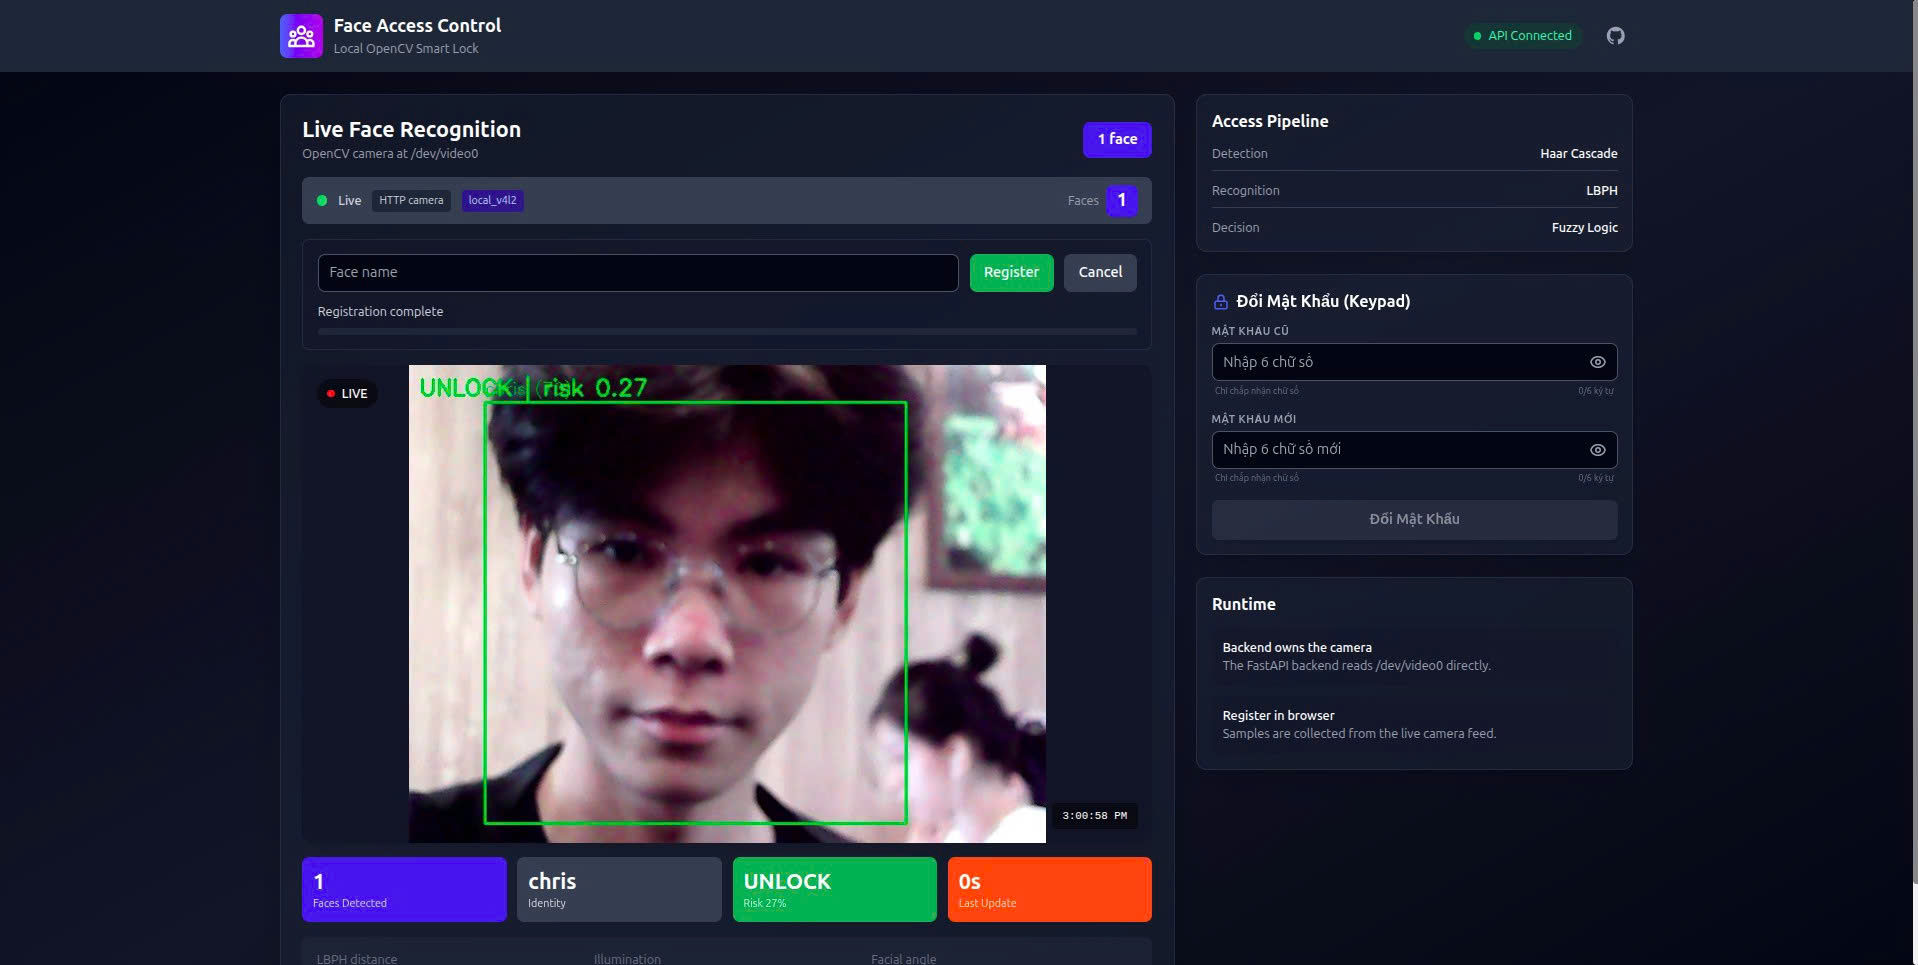
\includegraphics[width=\linewidth]{dashboard_nextjs.png}
    \caption{Kết quả giao diện live face recognition trên dashboard}
    \label{fig:frontend_result}
\end{figure}

\begin{figure}[H]
    \centering
    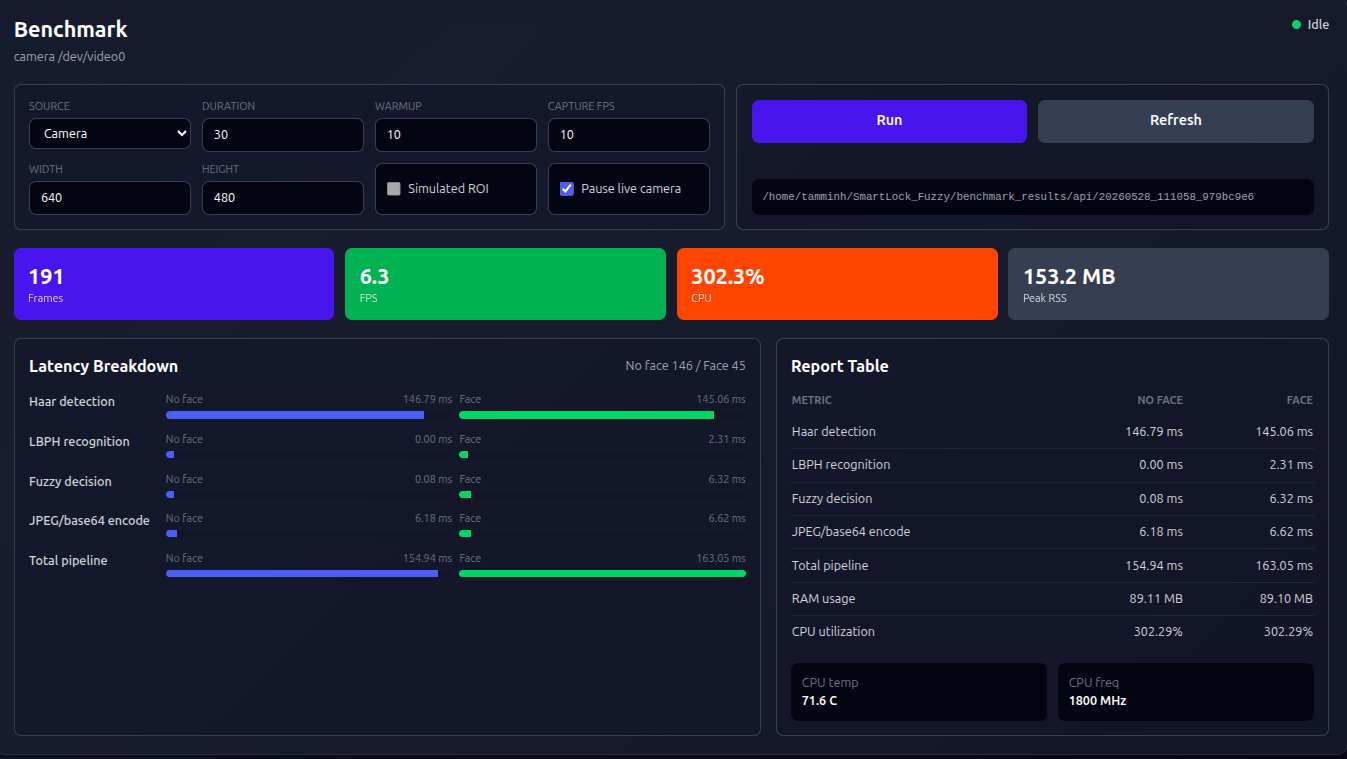
\includegraphics[width=\linewidth]{benchmark_ui.png}
    \caption{Giao diện benchmark hiển thị FPS, CPU, RAM và độ trễ từng bước}
    \label{fig:benchmark_ui_result}
\end{figure}

\subsection{Kết quả phần cứng}

Hệ thống đã được lắp trên Raspberry Pi cùng camera USB, keypad ma trận 4x4, OLED SSD1306 và servo. Ảnh ở Hình \ref{fig:hardware_connected_result} cho thấy cấu hình kết nối thực tế: camera gắn qua USB, keypad nối vào các chân GPIO hàng/cột, OLED nối qua SPI và servo nhận tín hiệu PWM từ GPIO18. Servo được cấp nguồn 5V ngoài và nối chung GND với Raspberry Pi để tránh sụt áp khi motor quay.

\begin{figure}[H]
    \centering
    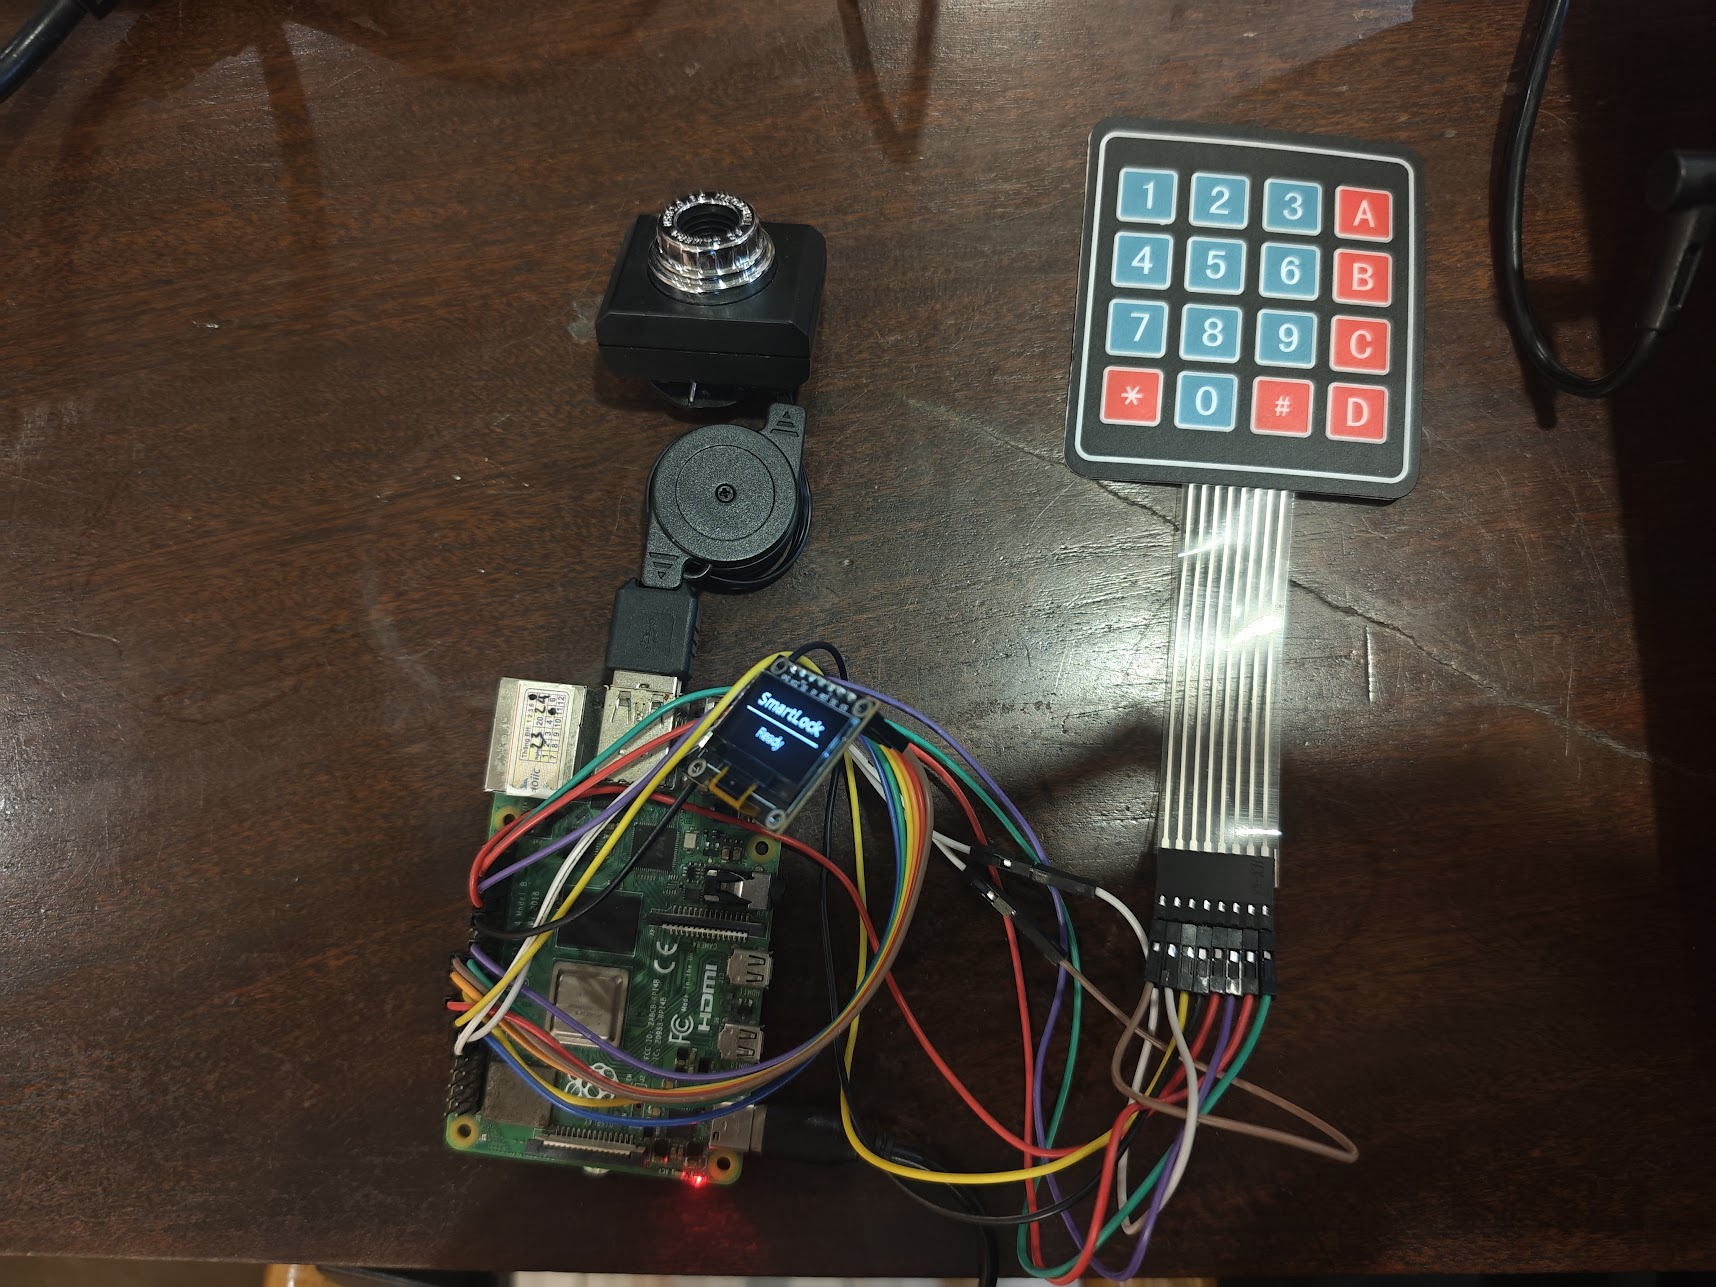
\includegraphics[width=\linewidth]{schematic_connected.png}
    \caption{Mạch phần cứng đã đấu nối trên Raspberry Pi}
    \label{fig:hardware_connected_result}
\end{figure}

Trong quá trình chạy thử, OLED hiển thị trạng thái \texttt{SmartLock Ready}; keypad được dùng cho kênh xác thực PIN; servo đóng vai trò cơ cấu chốt khóa. Phần mềm phần cứng đã bao gồm quét keypad bằng interrupt, chống dội phím, lockout sau nhiều lần nhập sai và đưa duty cycle servo về 0 sau khi quay để giảm rung.

\subsection{Benchmark và giới hạn kiểm chứng}

Benchmark được chạy trực tiếp trên thiết bị edge Raspberry Pi với camera \texttt{/dev/video0}, độ phân giải $640\times480$, FPS capture đặt 10, thời gian đo 60 giây và 20 frame warm-up. Tổng cộng script ghi nhận 489 frame, trong đó có 435 frame không có mặt và 54 frame có mặt; không có frame bị drop. Throughput trung bình đạt 8.14 FPS. Nhiệt độ CPU cuối quá trình đo là $67.7^\circ$C, xung CPU 1800 MHz và cờ throttling là \texttt{0x0}, cho thấy thiết bị không bị throttling trong lần đo này.

\begin{table}[H]
\centering
\caption{Kết quả benchmark pipeline trên Raspberry Pi}
\label{tab:benchmark_results}
\begin{tabular}{|l|c|c|}
\hline
\textbf{Chỉ số} & \textbf{Không có mặt} & \textbf{Có mặt} \\
\hline
Face detection latency & 111.26 ms & 108.43 ms \\
\hline
Face recognition latency & 0.00 ms & 2.15 ms \\
\hline
Fuzzy decision latency & 0.08 ms & 5.90 ms \\
\hline
JPEG/base64 encode latency & 5.91 ms & 6.34 ms \\
\hline
Total pipeline latency & 121.36 ms & 127.36 ms \\
\hline
RAM usage & 89.27 MB & 89.25 MB \\
\hline
CPU utilization & 319.07\% & 319.07\% \\
\hline
\end{tabular}
\end{table}

Kết quả cho thấy phần tốn thời gian nhất là Haar Cascade, chiếm hơn 100 ms mỗi frame ở cả hai trường hợp. Khi có khuôn mặt, hệ thống phát sinh thêm chi phí LBPH và fuzzy decision, nhưng tổng độ trễ chỉ tăng từ 121.36 ms lên 127.36 ms. Với throughput khoảng 8 FPS, pipeline đủ dùng cho kịch bản khóa cửa, nơi yêu cầu chính là phản hồi ổn định trong khoảng dưới một giây thay vì video FPS cao.

Các giới hạn hiện tại:

\begin{itemize}
    \item LBPH nhạy với điều kiện ánh sáng và chất lượng dữ liệu đăng ký.
    \item Fuzzy angle estimation chỉ dựa trên bất đối xứng sáng, chưa phải ước lượng pose thật.
    \item Mật khẩu keypad chưa được lưu bền vững qua các lần restart.
    \item CORS đang mở \texttt{allow\_origins=["*"]}, phù hợp demo nhưng cần siết lại nếu triển khai thật.
    \item Chưa có authentication cho API quản trị như đăng ký khuôn mặt hoặc đổi PIN.
\end{itemize}

\section{Kết luận}

\subsection{Kết quả đạt được}

Đề tài đã xây dựng được một hệ thống khóa cửa thông minh hoàn chỉnh ở mức prototype. Backend có thể đọc camera cục bộ, phát hiện khuôn mặt, nhận diện bằng LBPH, đánh giá rủi ro bằng fuzzy logic và cung cấp API cho dashboard. Hệ thống cũng hỗ trợ đăng ký khuôn mặt mới, huấn luyện lại model LBPH, đổi mật khẩu keypad và điều khiển phần cứng Raspberry Pi gồm keypad, OLED và servo.

Về mặt kiến trúc, hệ thống được tổ chức rõ thành các service độc lập: xử lý ảnh, fuzzy decision, đăng ký, camera worker, phần cứng và frontend. Cách chia này giúp dễ debug, dễ thay thế từng thành phần và phù hợp cho việc mở rộng sau này.

\subsection{Hạn chế}

\begin{itemize}
    \item Nhận diện LBPH còn phụ thuộc mạnh vào chất lượng mẫu đăng ký và điều kiện ánh sáng.
    \item Hệ thống mới xử lý một khuôn mặt lớn nhất, chưa hỗ trợ tình huống nhiều người đứng trước camera.
    \item OTP mới tồn tại ở mức action fuzzy, chưa có module gửi/kiểm tra OTP thật.
    \item API quản trị chưa có cơ chế xác thực người dùng.
    \item Mật khẩu keypad chưa được lưu vào file cấu hình hoặc cơ sở dữ liệu bền vững.
    \item Báo cáo cần bổ sung thêm ảnh phần cứng, ảnh dashboard và số liệu benchmark thực tế.
\end{itemize}

\subsection{Hướng phát triển}

\begin{itemize}
    \item Thay LBPH bằng mô hình embedding nhẹ như FaceNet/MobileFaceNet nếu thiết bị đủ tài nguyên.
    \item Bổ sung cơ chế lưu mật khẩu bền vững kèm salt thay vì chỉ SHA-256 trực tiếp.
    \item Thêm xác thực cho các API đăng ký và đổi mật khẩu.
    \item Hoàn thiện luồng OTP hoặc xác thực hai yếu tố thật.
    \item Lưu lịch sử truy cập vào SQLite hoặc một hệ thống log có cấu trúc.
    \item Chạy benchmark trên Raspberry Pi thật để chốt FPS, độ trễ và tài nguyên.
    \item Thêm test tự động cho registration, fuzzy decision, API schema và hardware mock.
\end{itemize}

\clearpage


% ===== REFERENCES =====
\begin{thebibliography}{99}

\bibitem{viola2001}
P. Viola and M. Jones,
``Rapid Object Detection using a Boosted Cascade of Simple Features,''
\textit{Proceedings of the IEEE Conference on Computer Vision and Pattern Recognition}, 2001.

\bibitem{lbph2006}
T. Ahonen, A. Hadid, and M. Pietikäinen,
``Face Description with Local Binary Patterns: Application to Face Recognition,''
\textit{IEEE Transactions on Pattern Analysis and Machine Intelligence}, vol. 28, no. 12, pp. 2037--2041, 2006.

\bibitem{opencv}
OpenCV,
``Open Source Computer Vision Library,''
\url{https://opencv.org/}

\bibitem{zadeh1965}
L. A. Zadeh,
``Fuzzy Sets,''
\textit{Information and Control}, vol. 8, no. 3, pp. 338--353, 1965.

\bibitem{mamdani1975}
E. H. Mamdani and S. Assilian,
``An experiment in linguistic synthesis with a fuzzy logic controller,''
\textit{International Journal of Man-Machine Studies}, vol. 7, no. 1, pp. 1--13, 1975.

\bibitem{fuzzylite}
FuzzyLite,
``FuzzyLite and pyfuzzylite fuzzy logic control libraries,''
\url{https://www.fuzzylite.com/}

\bibitem{fastapi}
FastAPI,
``FastAPI documentation,''
\url{https://fastapi.tiangolo.com/}

\bibitem{nextjs}
Vercel,
``Next.js documentation,''
\url{https://nextjs.org/docs}

\bibitem{raspberrypi}
Raspberry Pi Ltd.,
``Raspberry Pi Documentation,''
\url{https://www.raspberrypi.com/documentation/}

\bibitem{lumaoled}
Luma.OLED,
``luma.oled documentation,''
\url{https://luma-oled.readthedocs.io/}

\end{thebibliography}


% ===== APPENDIX =====
\appendix
\section{Phụ lục: Mã nguồn và lệnh chạy}

\subsection{Cấu trúc thư mục chính}

\begin{lstlisting}[language=bash, caption={Cấu trúc chính của project}, label={lst:project_structure}]
backend/
  main.py                     # FastAPI entrypoint
  routers/get_camera.py       # Camera latest/frame/history API cache
  services/
    local_camera.py           # Camera worker trung tam
    face_detection.py         # Haar + LBPH + quality metrics
    fuzzy_logic.py            # Wrapper fuzzy + fallback
    registration.py           # Thu mau va train LBPH
    hardware_io.py            # Keypad + servo
    oled_display.py           # SSD1306 OLED UI
  infra/fuzzy_controller.py   # Mamdani fuzzy controller

frontend/
  src/app/page.tsx
  src/components/
    LiveVideoStream.tsx
    PasswordChange.tsx
    Header.tsx

custom_models/                # Model artifacts
registered_faces/             # Mau dang ky, tao khi chay
\end{lstlisting}

\subsection{Lệnh chạy backend}

\begin{lstlisting}[language=bash, caption={Cài đặt và chạy backend}, label={lst:backend_run}]
python -m venv .venv
source .venv/bin/activate
pip install -r requirements.txt
python backend/main.py
\end{lstlisting}

Trên máy không phải Raspberry Pi, các thư viện GPIO/OLED có thể không import được. Khi chỉ benchmark phần pipeline, dùng script \texttt{backend/benchmark\_pipeline.py} vì script này mock phần cứng.

\subsection{Lệnh chạy frontend}

\begin{lstlisting}[language=bash, caption={Cài đặt và chạy frontend}, label={lst:frontend_run}]
cd frontend
npm install
cp .env.example .env.local
npm run dev
\end{lstlisting}

\subsection{Lệnh benchmark}

\begin{lstlisting}[language=bash, caption={Benchmark pipeline trên thiết bị edge}, label={lst:benchmark_run}]
python3 backend/benchmark_pipeline.py \
  --source camera \
  --camera /dev/video0 \
  --duration 60 \
  --warmup 20 \
  --width 640 \
  --height 480 \
  --capture-fps 10 \
  --output-dir benchmark_results/pi_camera
\end{lstlisting}

Script tự chia frame thành hai nhóm không có mặt và có mặt dựa trên kết quả Haar Cascade. Để điền đủ hai cột trong bảng báo cáo, có thể để camera trống trong một phần thời gian đo và đứng trước camera trong phần còn lại. Sau khi chạy, script sinh các file \texttt{summary.json}, \texttt{summary.md}, \texttt{summary\_table.tex} và \texttt{frames.csv}. File \texttt{summary\_table.tex} có thể dùng để điền bảng benchmark trong chương kết quả.

\subsection{Trích đoạn mã nguồn quan trọng}

\subsubsection{FastAPI entrypoint}
\lstinputlisting[
    language=Python,
    firstline=96,
    lastline=172,
    caption={FastAPI app, lifespan và API chính trong \texttt{backend/main.py}},
    label={lst:backend_main}
]{../backend/main.py}

\subsubsection{Camera router cache}
\lstinputlisting[
    language=Python,
    firstline=37,
    lastline=124,
    caption={Cache frame mới nhất trong \texttt{backend/routers/get\_camera.py}},
    label={lst:get_camera}
]{../backend/routers/get_camera.py}

\subsubsection{Camera worker}
\lstinputlisting[
    language=Python,
    firstline=85,
    lastline=207,
    caption={Vòng lặp xử lý camera trong \texttt{backend/services/local\_camera.py}},
    label={lst:local_camera_loop}
]{../backend/services/local_camera.py}

\subsubsection{Face detection và recognition}
\lstinputlisting[
    language=Python,
    firstline=75,
    lastline=160,
    caption={Phân tích khuôn mặt trong \texttt{backend/services/face\_detection.py}},
    label={lst:face_detection_analyze}
]{../backend/services/face_detection.py}

\subsubsection{Registration quality filter}
\lstinputlisting[
    language=Python,
    firstline=161,
    lastline=225,
    caption={Lọc chất lượng ảnh đăng ký trong \texttt{backend/services/face\_detection.py}},
    label={lst:registration_quality}
]{../backend/services/face_detection.py}

\subsubsection{Fuzzy decision wrapper}
\lstinputlisting[
    language=Python,
    firstline=49,
    lastline=109,
    caption={Wrapper đánh giá fuzzy trong \texttt{backend/services/fuzzy\_logic.py}},
    label={lst:fuzzy_wrapper}
]{../backend/services/fuzzy_logic.py}

\subsubsection{Fuzzy controller rule base}
\lstinputlisting[
    language=Python,
    firstline=115,
    lastline=192,
    caption={Tập luật fuzzy trong \texttt{backend/infra/fuzzy\_controller.py}},
    label={lst:fuzzy_rules}
]{../backend/infra/fuzzy_controller.py}

\subsubsection{Keypad và servo}
\lstinputlisting[
    language=Python,
    firstline=194,
    lastline=257,
    caption={Quét keypad trong \texttt{backend/services/hardware\_io.py}},
    label={lst:hardware_pin_servo}
]{../backend/services/hardware_io.py}

\subsubsection{Frontend live stream}
\lstinputlisting[
    language=Java,
    firstline=72,
    lastline=139,
    caption={Polling frame trong \texttt{frontend/src/components/LiveVideoStream.tsx}},
    label={lst:frontend_polling}
]{../frontend/src/components/LiveVideoStream.tsx}

\subsubsection{Đổi mật khẩu keypad}
\lstinputlisting[
    language=Java,
    firstline=50,
    lastline=64,
    caption={Request đổi mật khẩu trong \texttt{frontend/src/components/PasswordChange.tsx}},
    label={lst:password_change}
]{../frontend/src/components/PasswordChange.tsx}


\end{document}
